\documentclass[12pt]{article}

% Public portfolio edition: 12-point standard font, normal margins, standard
% spacing, and PDF output. Personal student identifiers and institutional
% email addresses are intentionally omitted.
\usepackage[T1]{fontenc}
\usepackage{mathptmx}
\usepackage[margin=1in]{geometry}
\usepackage{setspace}
\setstretch{1.15}

\usepackage{amsmath,amssymb}
\usepackage{graphicx}
\usepackage{subcaption}
\usepackage{float}
\usepackage{booktabs}
\usepackage{array}
\usepackage{enumitem}
\usepackage{needspace}
\usepackage{xcolor}
\usepackage{microtype}
\usepackage{fancyhdr}
\usepackage{tikz}
\usetikzlibrary{arrows.meta,positioning}
\usepackage[hidelinks]{hyperref}

\setlength{\parindent}{0.25in}
\setlength{\parskip}{0.25em}
\setlength{\textfloatsep}{12pt plus 2pt minus 2pt}
\setlength{\floatsep}{10pt plus 2pt minus 2pt}
\setlength{\intextsep}{10pt plus 2pt minus 2pt}

\pagestyle{fancy}
\setlength{\headheight}{15pt}
\fancyhf{}
\fancyhead[L]{EECS 3404 Final Project}
\fancyhead[R]{Forecast-Driven Elevator Group Control}
\fancyfoot[C]{\thepage}
\renewcommand{\headrulewidth}{0.4pt}

\newcommand{\projecttitle}{Forecast-Driven Elevator Group Control Under Traffic Drift}
\newcommand{\projectsubtitle}{A Digital-Twin Comparison Study}

\newcommand{\makeprojecttitle}{%
  \begin{center}
    {\LARGE\bfseries \projecttitle\par}
    \vspace{0.25em}
    {\large \projectsubtitle\par}
    \vspace{0.65em}
    \begingroup
    \setstretch{1.0}
    \textbf{Hannah Abedin}\\[0.35em]
    \textbf{Erfan Razmand}
    \par
    \endgroup
    \vspace{0.55em}
    EECS 3404: Applied Machine Learning\\
    York University\\
    August 2026
  \end{center}
  \vspace{0.35em}
}

\begin{document}

\makeprojecttitle

\begin{abstract}
Elevator group control is an operational machine-learning problem in which
small forecasting improvements do not necessarily translate into better
passenger service. This project develops a deterministic digital twin of a
15-floor office building with four elevators and evaluates whether
short-horizon, per-floor passenger-demand forecasts can improve idle-car
positioning under normal traffic and distribution shift. Leakage-safe temporal
features and independent building-day splits are used to compare mean,
historical, persistence, Ridge, Random Forest, and from-scratch Elman recurrent
forecasters. The controllers are evaluated against nearest-car and static
zoning using passenger waiting time, tail wait, long-wait rate, floor fairness,
and elevator movement. On the untouched in-distribution holdout, Random Forest
reduces per-floor mean absolute error from 0.897 to 0.868 relative to the
historical baseline, with a paired 95\% bootstrap interval of 0.011 to 0.046
passengers for the reduction. However, its forecast-driven controller changes
mean wait from 16.023 to 16.038 seconds, worsens P95 wait by 1.168 seconds, and
increases movement by 1.75\%. These results demonstrate that better offline
prediction does not guarantee operational value. The primary engineering
limitation is the greedy positioning layer, which lacks destination-aware
routing, capacity planning, and an explicit tail-service objective.
\end{abstract}

\noindent\textbf{Keywords:} applied machine learning, elevator group control,
demand forecasting, digital twin, Random Forest, recurrent neural network,
distribution shift, uncertainty, simulation

\vspace{0.75em}
\hrule
\vspace{0.75em}

\section{Introduction}

Busy multi-elevator buildings face a sequential resource-allocation problem:
cars must respond to current calls while anticipating where future passengers
will arrive. Conventional nearest-car dispatch is reactive, whereas
forecast-driven positioning can move service-idle cars toward predicted demand.
The possible benefit comes with a cost: speculative movement may waste energy,
remove capacity from the wrong region, or increase tail waiting time when
traffic changes unexpectedly.

This project asks whether short-horizon spatial demand forecasts provide
measurable operational value when embedded in an elevator controller. The
study deliberately evaluates forecasting and control as separate layers. This
distinction is central to the final result: Random Forest improves prediction
accuracy on independent days, but the locked greedy controller does not convert
that gain into a reliable waiting-time improvement.

Elevator group control is a stochastic sequential decision problem; prior work
has studied it with simulated multi-agent reinforcement learning
\cite{crites1998elevator}. This project does not claim a new forecasting
algorithm; its contribution is an auditable separation of supervised demand
forecasting from transparent idle-car positioning, testing whether offline
prediction gains change actions and passenger service under drift.

% Evidence audit: report/evidence/02_problem_definition.md
\section{Problem Definition and Study Scope}
\label{sec:problem-definition}

\subsection{System Boundary}

The project studies forecast-assisted \emph{idle-car positioning}, not the
design of a complete commercial elevator controller. The controlled setting is
a seeded digital twin of a 15-floor office building with four identical
elevators. Each simulated session generates anonymous passenger trips, where a
trip records an arrival time, an origin floor, and a different destination
floor. All policy variants receive the same trips within a building day.

Floors are indexed from 0 to 14, with floor 0 representing the lobby. The
fixed physical and decision scope is summarized in
Table~\ref{tab:locked-scope}.

\begin{table}[H]
  \centering
  \caption{Locked experimental scope used for the primary comparison.}
  \label{tab:locked-scope}
  \begin{tabular}{@{}lr@{}}
    \toprule
    Quantity & Locked value \\
    \midrule
    Building floors & 15 \\
    Elevators & 4 \\
    Car capacity & 12 passengers \\
    Traffic-generation duration & 75 minutes \\
    Primary forecast horizon & 2 minutes \\
    Forecast-positioning interval & 5 minutes \\
    Long-wait threshold & 60 seconds \\
    Development movement budget & 5\% above nearest-car \\
    \bottomrule
\end{tabular}
\end{table}

\Needspace{7\baselineskip}
The reactive hall-call assignment policy is held constant across comparisons.
It assigns calls using car distance, queued work, occupancy, direction, and
same-floor availability. The experimental intervention changes only what a
service-idle elevator does before the next call arrives: the baseline leaves
it in place, while the forecast-aware policy may give it a temporary parking
target. Passenger service always takes priority over speculative positioning.
This boundary isolates the incremental value of demand forecasting without
attributing improvements from an unrelated dispatch algorithm to the learned
model.

\subsection{Forecasting Task}

Let $A_{d,\tau,f}$ be the number of passengers who arrive on building day $d$
during minute $\tau$ with origin floor $f$. For a forecast issued at minute
$t$, the $H$-minute target is

\begin{equation}
  y_{d,t,f}^{(H)} = \sum_{\tau=t}^{t+H-1} A_{d,\tau,f},
  \qquad f\in\{0,\ldots,F-1\}.
  \label{eq:forecast-target}
\end{equation}

The model produces the multi-output prediction

\begin{equation}
  \widehat{\mathbf{y}}_{d,t}^{(H)}
  = g(\mathbf{x}_{d,t})
  = \left[\widehat{y}_{d,t,0}^{(H)},\ldots,
  \widehat{y}_{d,t,F-1}^{(H)}\right],
  \label{eq:forecast-vector}
\end{equation}

where every element of $\mathbf{x}_{d,t}$ is available strictly before minute
$t$. The primary task fixes $F=15$ and $H=2$. Its day-level error for model
$m$ is the mean absolute error over all eligible forecast minutes $\mathcal{T}_d$
and floors:

\begin{equation}
  \operatorname{MAE}_{d}^{(m)} =
  \frac{1}{|\mathcal{T}_d|F}
  \sum_{t\in\mathcal{T}_d}\sum_{f=0}^{F-1}
  \left|\widehat{y}_{d,t,f}^{(m)}-y_{d,t,f}\right|.
  \label{eq:day-forecast-mae}
\end{equation}

Random Forest is the locked learned challenger and the historical mean is the
primary forecasting baseline. Per-floor mean, persistence, Ridge regression,
and an Elman recurrent neural network remain secondary comparisons rather than
substitutes for the locked primary contrast.

\subsection{Operational Task}

Let $a_{d,i}$ be passenger $i$'s arrival time and let $b_{d,i}^{(\pi)}$ be the
time that passenger boards under policy $\pi$. Passenger wait is
$w_{d,i}^{(\pi)}=b_{d,i}^{(\pi)}-a_{d,i}$, and the day-level mean wait is

\begin{equation}
  W_d^{(\pi)} = \frac{1}{N_d}\sum_{i=1}^{N_d}w_{d,i}^{(\pi)},
  \label{eq:day-mean-wait}
\end{equation}

where $N_d$ is the number of passengers generated on day $d$. The primary
operational baseline, $\pi_{\mathrm{NC}}$, combines nearest-car assignment with
no idle repositioning. The challenger, $\pi_{\mathrm{RF}}$, retains the same
assignment logic but uses Random Forest forecasts to position service-idle
cars every five minutes. The paired day-level benefit is defined as

\begin{equation}
  \Delta_W = \frac{1}{D}\sum_{d=1}^{D}
  \left(W_d^{(\pi_{\mathrm{NC}})}-W_d^{(\pi_{\mathrm{RF}})}\right),
  \label{eq:paired-wait-effect}
\end{equation}

so a positive value means that forecast-aware positioning reduces mean wait.
The day, rather than the passenger or forecast minute, is the independent
evaluation unit. Uncertainty is therefore quantified with a paired 95\%
bootstrap interval \cite{efron1979bootstrap} over building days using 2,000
resamples. This pairing
preserves the common passenger stream and avoids treating correlated
passengers from the same simulated session as independent observations.

\subsection{Locked Research Questions}

The final protocol fixes four questions before the final seed was revealed:

\begin{enumerate}[label=\textbf{RQ\arabic*:}, leftmargin=3.5em]
  \item Does Random Forest reduce two-minute per-floor demand MAE relative to
  the historical-mean baseline on independent in-distribution building days?
  \item Does Random Forest-driven idle-car positioning reduce mean passenger
  wait relative to nearest-car assignment with idle cars left in place?
  \item Is any mean-wait benefit acceptable when evaluated beside P95 wait,
  the proportion of waits exceeding 60 seconds, floor-level service fairness,
  and elevator movement?
  \item How do the forecasting and controller conclusions change under an
  unseen event surge and a 1.5$\times$ demand-intensity shift?
\end{enumerate}

\subsection{Directional Hypotheses and Interpretation Criteria}

\paragraph{Forecasting hypothesis ($H_{\mathrm{F}}$).}
On the in-distribution final holdout, Random Forest will have lower day-level
per-floor MAE than the historical-mean model. Its paired effect is

\begin{equation}
  \Delta_{\mathrm{MAE}} = \frac{1}{D}\sum_{d=1}^{D}
  \left(\operatorname{MAE}_{d}^{(\mathrm{Hist})}
  -\operatorname{MAE}_{d}^{(\mathrm{RF})}\right),
  \label{eq:paired-forecast-effect}
\end{equation}

with positive values favoring Random Forest.

\paragraph{Controller hypothesis ($H_{\mathrm{C}}$).}
On the same in-distribution holdout, Random Forest positioning will produce
$\Delta_W>0$ relative to nearest-car with no repositioning. A favorable mean
alone is not interpreted as a safe operational improvement: P95 wait,
long-wait rate, floor fairness, and movement are reported beside the primary
effect. The predeclared development movement budget is a 5\% increase relative
to nearest-car.

The stress evaluations answer RQ4 but do not redefine either primary
hypothesis. An unseen-surge set and a separate 1.5$\times$-demand set are
reported as distribution-shift tests, including results that contradict the
in-distribution direction. Throughout the report, effect magnitudes and their
paired day-level intervals are emphasized rather than declaring success from a
single favorable aggregate.

% Evidence audit: report/evidence/03_simulator.md
\section{Digital-Twin Simulator Design and Assumptions}
\label{sec:simulator}

\subsection{Purpose and Architecture}

The simulator provides a controlled counterfactual environment in which every
elevator policy can be evaluated on the same passenger demand. We use the term
\emph{digital twin} in this limited experimental sense: the software is an
executable state model of a multi-elevator building, but it is not synchronized
with or calibrated to a particular physical building. Its purpose is to expose
the interaction between demand forecasts and controller decisions while
holding the passenger stream and mechanical assumptions fixed.

The simulator separates demand, control, and evaluation. A generated
\texttt{DayData} object contains a source passenger trip stream that is treated
as immutable, plus
per-minute origin and destination counts. Each policy run deep-copies the
passengers, initializes four cars at the lobby, and evolves only its private
elevator and passenger state. The resulting boarding times, drop-off times,
and car counters are converted to service and movement metrics after the run.
This design prevents one policy from changing the demand or state observed by
another policy.

Figure~\ref{fig:simulation-loop} summarizes initialization and the exact order
used at each simulated second.

\begin{figure}[H]
  \centering
  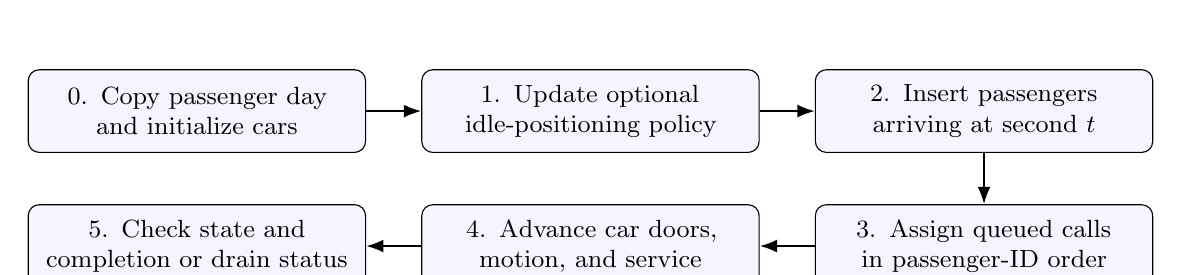
\begin{tikzpicture}[
    node distance=0.65cm and 0.70cm,
    stage/.style={
      draw,
      rounded corners,
      align=center,
      minimum height=1.05cm,
      text width=4.05cm,
      font=\small,
      fill=blue!4
    },
    flow/.style={-{Latex[length=2.2mm]},thick}
  ]
    \node[stage] (copy) {0. Copy passenger day\\and initialize cars};
    \node[stage,right=of copy] (position) {1. Update optional\\idle-positioning policy};
    \node[stage,right=of position] (arrivals) {2. Insert passengers\\arriving at second $t$};
    \node[stage,below=of arrivals] (assign) {3. Assign queued calls\\in passenger-ID order};
    \node[stage,left=of assign] (tick) {4. Advance car doors,\\motion, and service};
    \node[stage,left=of tick] (verify) {5. Check state and\\completion or drain status};
    \draw[flow] (copy) -- (position);
    \draw[flow] (position) -- (arrivals);
    \draw[flow] (arrivals) -- (assign);
    \draw[flow] (assign) -- (tick);
    \draw[flow] (tick) -- (verify);
  \end{tikzpicture}
  \par\smallskip
  {\footnotesize Steps 1--5 repeat at $t+1$ unless all passengers are served.}
  \caption{Simulator initialization and second-by-second execution order. A
  newly assigned passenger cancels speculative parking, so passenger service
  overrides forecast-driven positioning.}
  \label{fig:simulation-loop}
\end{figure}

\subsection{State Representation}

Three explicit state objects make transitions auditable. A passenger stores a
unique ID, arrival second, origin, destination, assigned car, boarding time,
and drop-off time. Its lifecycle is

\begin{equation}
  \text{not arrived}\;\longrightarrow\;\text{unassigned}
  \;\longrightarrow\;\text{waiting}
  \;\longrightarrow\;\text{onboard}
  \;\longrightarrow\;\text{completed}.
  \label{eq:passenger-lifecycle}
\end{equation}

Capacity overflow adds one permitted backward transition: a passenger who
cannot board is removed from the car's waiting set and returned to the global
unassigned queue. A passenger can never occupy more than one of the
unassigned, waiting, or onboard states.

An elevator stores its current floor, direction, passenger-service stops,
optional parking target, assigned waiting passengers, onboard passengers,
door and motion timers, and counters for floors travelled, stops, reversals,
and maximum load. A passenger-service stop has priority over a parking target.
The final \texttt{SimulationResult} contains the completed passenger copies and
terminal elevator states; the original generated day remains unchanged and
can therefore be reused for paired policy comparisons.

\subsection{Discrete-Time Execution}

The engine advances in one-second increments. At second $t$, it performs the
following operations in order:

\begin{enumerate}[leftmargin=1.7em,itemsep=0.25em,topsep=0.35em]
  \item If traffic generation is still active, invoke the optional positioning
  policy. The locked forecast-aware controller acts only at its five-minute
  decision times.
  \item Add all passengers whose recorded arrival time equals $t$ to the
  unassigned queue.
  \item Process unassigned passenger IDs deterministically and request an
  elevator from the common assignment policy. A successful assignment adds
  the origin as a service stop and clears that car's speculative parking
  target.
  \item Advance each elevator. An active door timer is processed first, then
  an active movement timer. Otherwise, the car serves its current floor or
  selects its next passenger-service stop; a parking target is considered only
  when no passenger-service stops remain.
  \item Optionally evaluate the full system invariants. After the 75-minute
  arrival period, terminate once every passenger has been dropped off.
\end{enumerate}

The fixed kinematic model uses two seconds per travelled floor and a four-second
door cycle. When a car serves a floor, drop-offs occur first. Waiting passengers
are then ordered by arrival time and passenger ID and board up to the remaining
capacity. Their destinations are added to the service-stop set only after
boarding. Boarding and exiting are treated as instantaneous events whose shared
time cost is represented by the door cycle.

When multiple stops exist, a moving car continues in its current direction
until no stop remains ahead, then reverses. A stationary car selects the
nearest service stop; floor ID resolves a stop tie, while elevator ID resolves
an assignment tie. Destination information affects the route after boarding
but does not enter the nearest-car hall-call assignment score.

\subsection{Termination and Software Verification}

Passenger generation ends after 75 minutes, but a run continues for a drain
period of at most 30 additional minutes. Forecast-based positioning is disabled
during this drain. If any passenger lacks a drop-off time at the hard limit,
the simulator raises an error rather than silently reporting metrics from an
incomplete run.

The implementation combines local validation with a global invariant checker.
The latter is enabled in targeted simulator tests and can be activated after
every simulated second. Table~\ref{tab:simulator-invariants} connects the main
failure risks to their enforcement mechanisms.

\begin{table}[htbp]
  \centering
  \caption{Simulator validity properties and enforcement mechanisms.}
  \label{tab:simulator-invariants}
  \begin{tabular}{@{}>{\raggedright\arraybackslash}p{0.32\textwidth}
    >{\raggedright\arraybackslash}p{0.60\textwidth}@{}}
    \toprule
    Property & Enforcement \\
    \midrule
    Valid time and floors & Reject negative times, equal origin/destination,
      out-of-building floors, and illegal movement. \\
    Passenger conservation & Require generated event counts to match both
      origin and destination matrices; reject lost or duplicated state. \\
    Temporal order & Reject boarding before arrival and drop-off before
      boarding. \\
    Capacity & Prevent assignment to a full car; board only available places
      and return overflow to the unassigned queue. \\
    Counterfactual parity & Deep-copy the same source day for every policy and
      verify deterministic repeated outcomes. \\
    Complete service & Continue through the drain period and fail the run if
      any passenger remains unserved. \\
    \bottomrule
  \end{tabular}
\end{table}

The targeted entity and simulator tests cover hand-calculated travel timing,
capacity overflow, direction reversal, drain behavior, source-day immutability,
identical demand across policies, deterministic replay, and forecast-only
parking. All 17 targeted tests passed when this section was prepared. In the
untouched final run, all passengers were served and the recorded peak load did
not exceed the configured capacity.

\subsection{Assumptions and Validity Boundary}

The simplifications in Table~\ref{tab:simulator-limitations} make the system
reproducible and computationally manageable, but they also define what the
experiment cannot establish.

\begin{table}[htbp]
  \centering
  \caption{Major simulator simplifications and their implications.}
  \label{tab:simulator-limitations}
  \begin{tabular}{@{}>{\raggedright\arraybackslash}p{0.29\textwidth}
    >{\raggedright\arraybackslash}p{0.63\textwidth}@{}}
    \toprule
    Simplification & Implication \\
    \midrule
    Homogeneous cars and fixed motion & Acceleration, deceleration, leveling,
      door obstruction, and car-specific performance are folded into fixed
      travel and door constants. \\
    Simplified passenger behavior & Passengers never abandon the queue, choose
      stairs, reserve capacity, or react strategically to visible car state. \\
    Normal operating mode only & Failures, maintenance, freight, accessibility
      priority, emergency calls, and fire-service modes are not modeled. \\
    Movement proxy & Floors travelled represents relative wear and energy cost;
      it is not a calibrated estimate of electrical consumption. \\
    Synthetic demand & Results support causal comparisons inside the simulator,
      not guaranteed performance in a real building. \\
    \bottomrule
  \end{tabular}
\end{table}

Accordingly, the strongest valid conclusion is comparative: under identical
synthetic traffic and the stated mechanics, one policy changes passenger
service and movement relative to another. Deployment claims would require
calibration against measured arrival patterns, origin-destination flows,
travel and door times, and the constraints of a real certified controller.

% Evidence audit: report/evidence/04_data_pipeline.md
\section{Synthetic Data, Features, and Leakage Prevention}
\label{sec:data-pipeline}

\subsection{Data Source and Traffic Generator}

No real passenger records are used. Instead, a seeded stochastic generator
creates independent 75-minute building days with passenger arrival time,
origin floor, and destination floor. Synthetic data make controlled
counterfactual comparisons and deliberate stress tests possible without
privacy concerns. They do not, however, establish that the simulated traffic
distribution matches a particular building.

For day $d$ and minute $t$, the number of new passengers is sampled as

\begin{equation}
  N_{d,t}\sim\operatorname{Poisson}(\lambda_{d,t}), \qquad
  \lambda_{d,t}=r_s(u_t)c_d z_{d,t}m_d,
  \label{eq:arrival-process}
\end{equation}

where $u_t=t/(T-1)$ is normalized session time, $r_s$ is the scenario-specific
base rate, $c_d\sim\operatorname{Uniform}(0.80,1.20)$ is a day-level scale, and
$m_d$ is an experimental demand multiplier. Short-term temporal correlation
is introduced through

\begin{equation}
  z_{d,t}=\operatorname{clip}
  \left(0.78z_{d,t-1}+0.22\epsilon_{d,t},\,0.60,\,1.55\right),
  \quad
  \epsilon_{d,t}\sim\operatorname{LogNormal}
  \left(-\tfrac{1}{2}(0.18)^2,0.18\right),
  \label{eq:latent-intensity}
\end{equation}

initialized from $z=1$. Each sampled passenger receives a uniformly random
arrival second within its minute. A day-specific log-normal vector supplies
heterogeneous upper-floor popularity, after which the scenario rules in
Table~\ref{tab:traffic-scenarios} sample the origin and destination. Trips with
equal origin and destination are rejected by construction.

\begin{table}[htbp]
  \centering
  \caption{Traffic scenarios implemented by the synthetic generator. The
  surge scenario is reserved for out-of-distribution evaluation.}
  \label{tab:traffic-scenarios}
  \begin{tabular}{@{}>{\raggedright\arraybackslash}p{0.15\textwidth}
    >{\raggedright\arraybackslash}p{0.34\textwidth}
    >{\raggedright\arraybackslash}p{0.43\textwidth}@{}}
    \toprule
    Scenario & Base arrival rate $r_s(u)$ & Origin-destination structure \\
    \midrule
    Morning & $7+11e^{-((u-0.38)/0.22)^2}$ & 84\% lobby-to-upper,
      10\% upper-to-lobby, and 6\% inter-floor. \\
    Lunch & $6+9e^{-((u-0.50)/0.25)^2}$ & Before $u=0.48$, 68\%
      upper-to-lobby; from $u=0.48$, 68\% lobby-to-upper. The remaining
      traffic is reverse-flow or inter-floor. \\
    Evening & $7+11e^{-((u-0.62)/0.22)^2}$ & 80\% upper-to-lobby,
      10\% lobby-to-upper, and 10\% inter-floor. \\
    Mixed & $7+3(0.5+0.5\sin(2\pi u))$ & 30\% lobby-to-upper,
      30\% upper-to-lobby, and 40\% inter-floor. \\
    Surge & 20 for $0.34\leq u<0.72$; otherwise 7 & A random upper meeting
      floor receives 74\% of trips during the inbound event window and is the
      origin of 74\% during the outbound window. \\
    \bottomrule
  \end{tabular}
\end{table}

Passenger events are sorted by arrival time and assigned unique IDs. The same
events are then aggregated into minute-by-floor origin and destination count
matrices. Automated conservation checks require the two matrices to contain
exactly the generated number of passengers. Fixed seeds make the study
reproducible without removing within-day or between-day stochastic variation.

\subsection{Partitioning and Data Audit}

The unit of partitioning is a complete building day. Minute-level rows from a
day never appear in more than one split, and the training and validation seed
sets are disjoint. The development audit generated only the 40 training and
12 validation days; it did not materialize the final seeds. Table~\ref{tab:data-partitions}
summarizes the data used by the primary two-minute forecasting task. Because a
75-minute day supplies eligible target minutes 10 through 73, each complete
day contributes 64 examples.

\begin{table}[H]
  \centering
  \caption{Whole-day partitions for the primary two-minute forecast. Final
  partitions remained sealed during development.}
  \label{tab:data-partitions}
  \begin{tabular}{@{}lrrrl@{}}
    \toprule
    Partition & Days & Passengers & Examples & Use \\
    \midrule
    Training & 40 & 30,448 & 2,560 & Fit models and preprocessing \\
    Validation & 12 & 9,109 & 768 & Select and diagnose \\
    Final in-distribution & 20 & -- & 1,280 & Locked primary evaluation \\
    Final unseen surge & 8 & -- & 512 & Novel-pattern stress test \\
    Final 1.5$\times$ demand & 8 & -- & 512 & Intensity-shift stress test \\
    \bottomrule
  \end{tabular}
\end{table}

The training and validation audit found the intended traffic signatures. In
training data, the lobby was the origin of 83.8\% of morning trips and the
destination of 79.6\% of evening trips. Mean demand ranged from 8.14
passengers per minute for mixed traffic to 11.32 for evening traffic. The
corresponding validation rates and directional shares were similar, providing
no evidence of an accidental development split shift. Figure~\ref{fig:traffic-audit}
shows the audited temporal, daily-count, floor, and origin-destination views.

\begin{figure}[H]
  \centering
  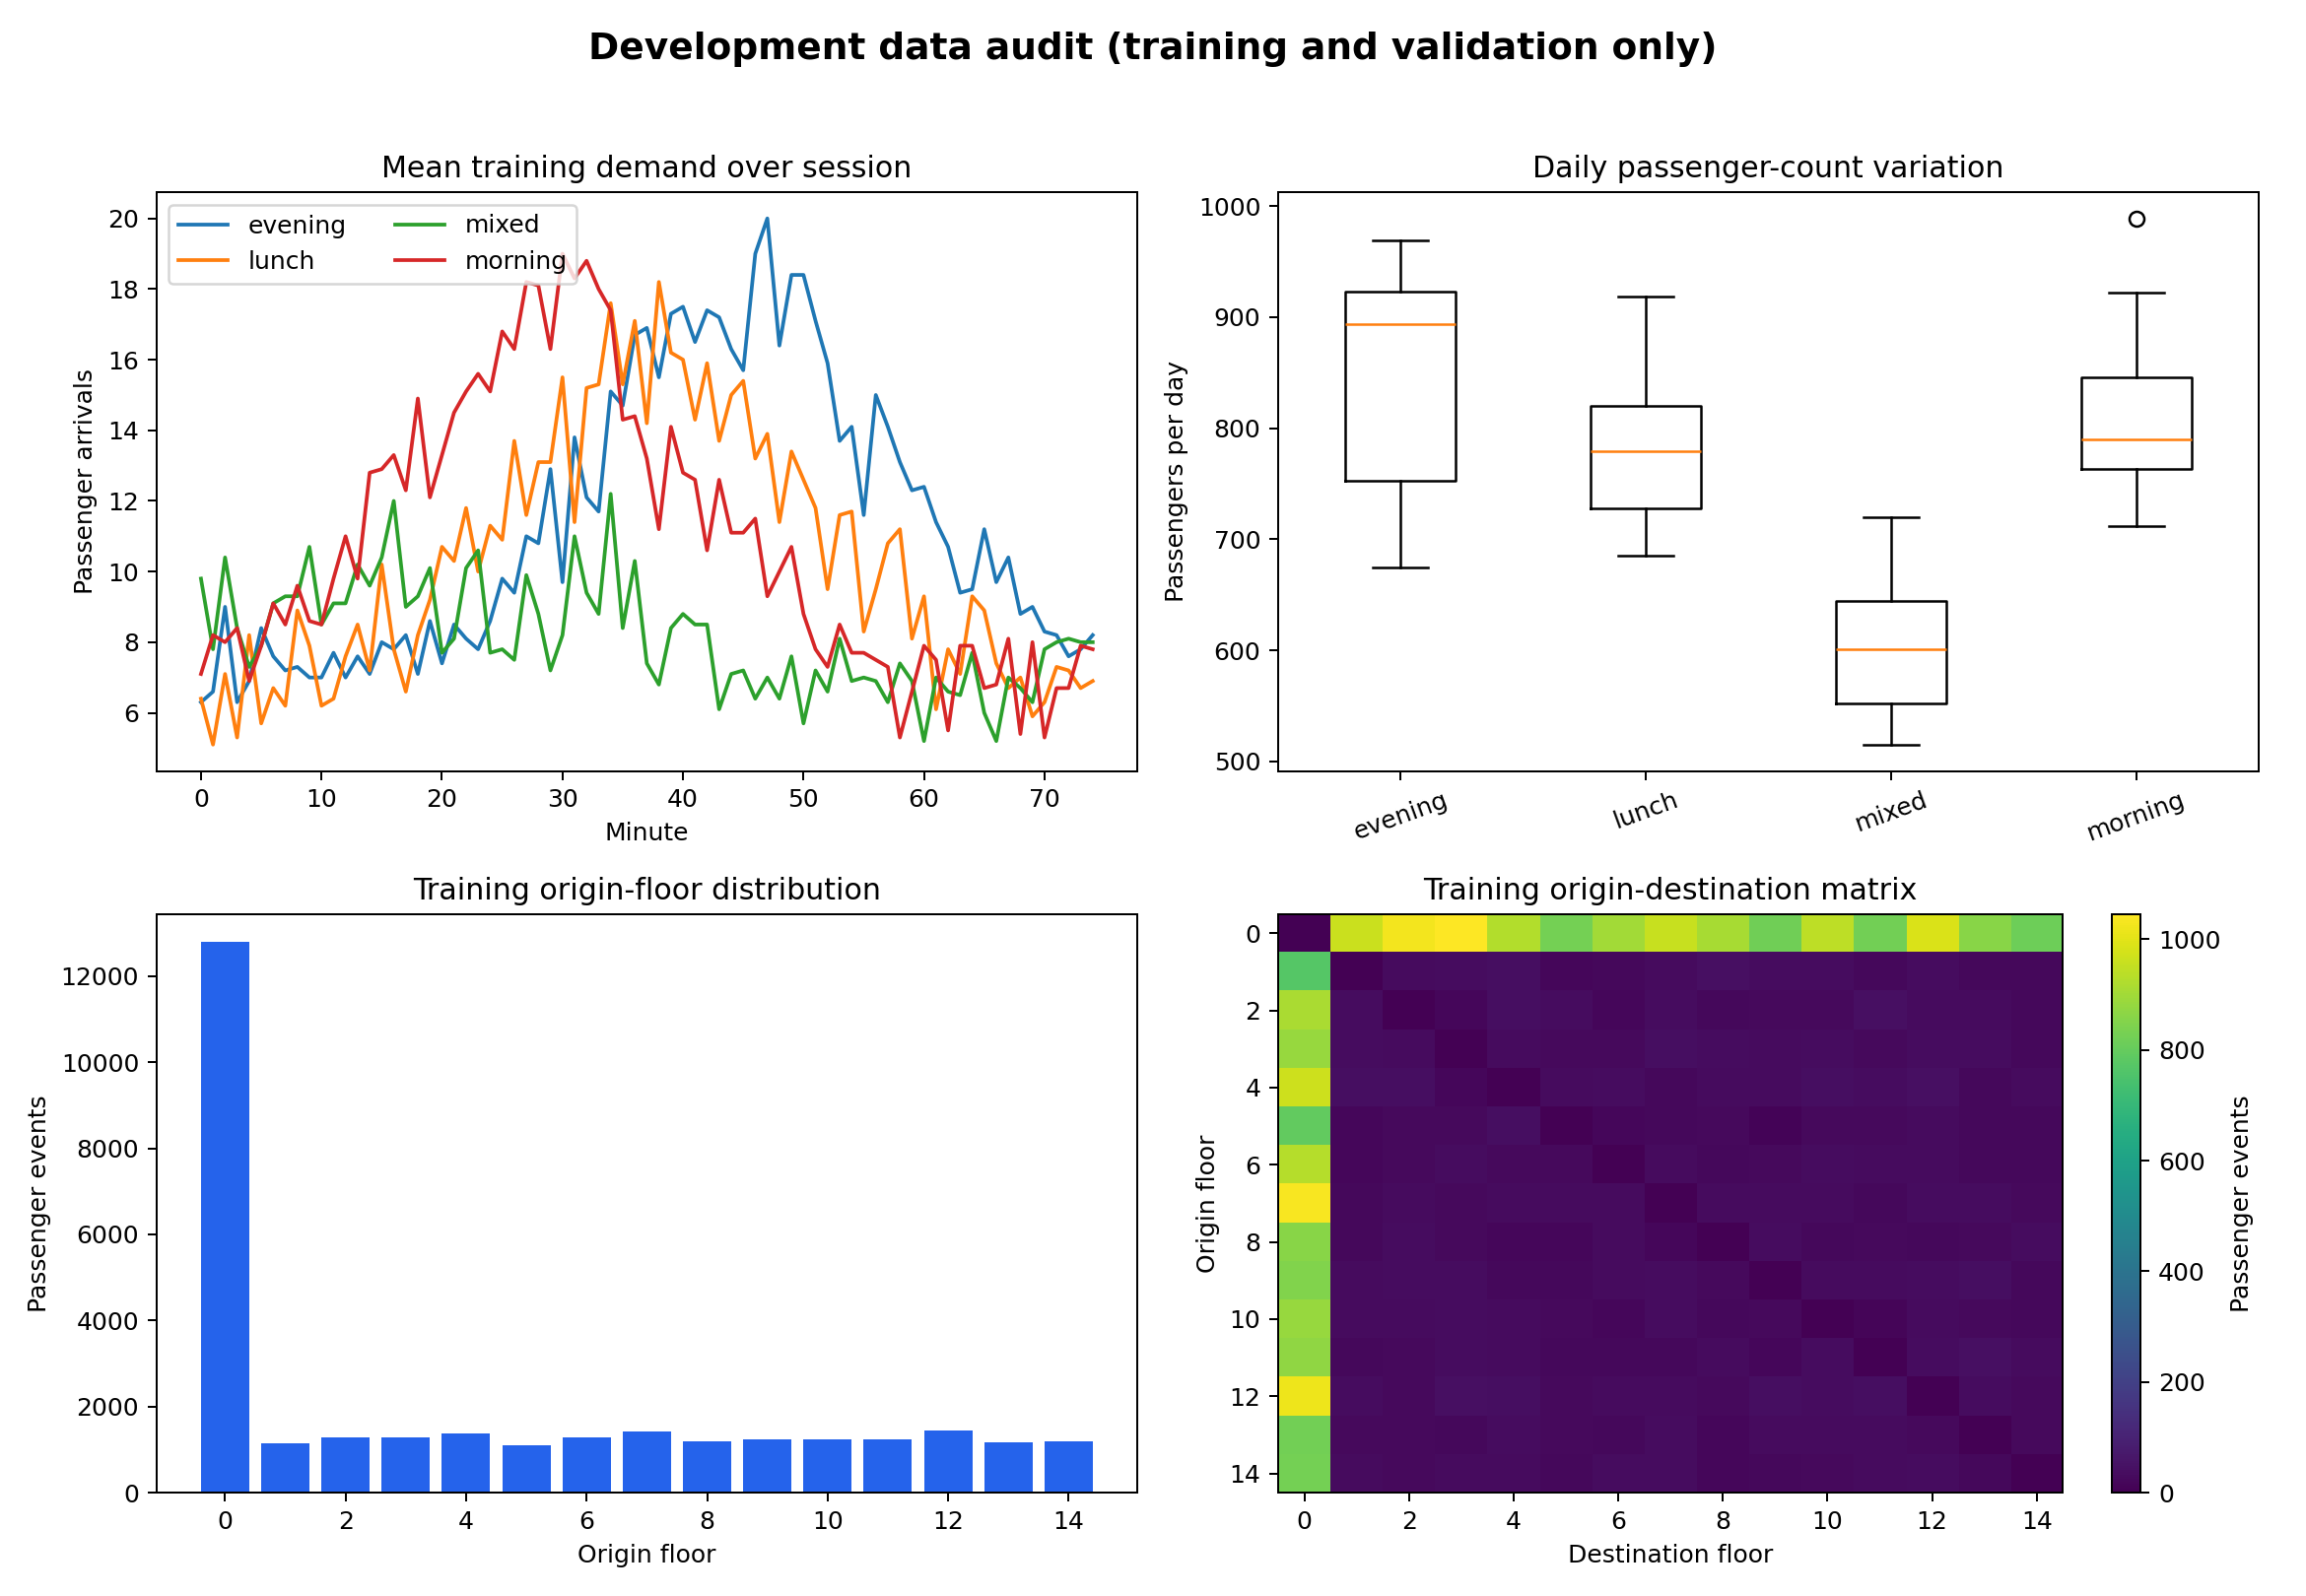
\includegraphics[width=0.96\textwidth]{../results/figures/traffic_audit.png}
  \caption{Training and validation traffic audit. The panels verify distinct
  scenario time profiles, plausible between-day count variation, floor-demand
  heterogeneity, and the intended origin-destination structure.}
  \label{fig:traffic-audit}
\end{figure}

\subsection{Tabular Features and Forecast Targets}

For target minute $t$, every tabular predictor is computed from indices
strictly less than $t$. The target is the 15-floor vector in
Equation~\ref{eq:forecast-target}. The primary horizon $H=2$ counts passenger
origins over $[t,t+2)$, while secondary datasets with $H\in\{1,5\}$ support
horizon-sensitivity analysis. Table~\ref{tab:feature-groups} accounts for all
101 input columns.

\begin{table}[H]
  \centering
  \caption{Feature groups for the 15-floor tabular forecasting models.}
  \label{tab:feature-groups}
  \begin{tabular}{@{}>{\raggedright\arraybackslash}p{0.31\textwidth}
    r>{\raggedright\arraybackslash}p{0.52\textwidth}@{}}
    \toprule
    Feature group & Count & Construction \\
    \midrule
    Time position & 3 & Sine and cosine of clock time plus elapsed-session
      fraction. \\
    Recent total arrivals & 4 & Building-wide origin counts over the previous
      1, 3, 5, and 10 minutes. \\
    Normal-regime indicator & 4 & One-hot values for morning, lunch, evening,
      and mixed traffic. \\
    Per-floor origin history & 60 & Fifteen floors times the previous 1, 3, 5,
      and 10-minute counts. \\
    Per-floor destination history & 15 & Per-floor requested-destination counts
      over the previous 3 minutes. \\
    Per-floor trend & 15 & Last-minute origin count minus the average of the
      preceding two minutes. \\
    \midrule
    Total & 101 & All columns are numeric, finite, and available before the
      target window under the stated availability assumptions. \\
    \bottomrule
  \end{tabular}
\end{table}

The Elman recurrent model receives an aligned representation rather than the
engineered 101-column vector. Each example contains the preceding 10 minutes
as a $10\times37$ array: 15 origin counts, 15 destination counts, three time
features, and four normal-regime indicators per step. Its input covers
$[t-10,t)$ and uses the same $[t,t+2)$ target as the tabular models. Sequence
construction is performed inside each day, so no sequence crosses a partition
or day boundary.

\subsection{Preprocessing and Availability Assumptions}

The generated count matrices are complete, so no missing-value imputation is
applied. Ridge uses predictor means and scales fitted on training rows, whereas
Random Forest uses the unscaled numeric features. The recurrent model estimates
input and target normalization statistics only from training sequences, reuses
them for validation and final inputs, and inverse-transforms its outputs. All
methods clip negative forecasts to zero.

The four scenario indicators describe only normal training regimes. An unseen
surge receives an all-zero vector rather than a category learned from final
data. A real installation would need a calendar rule or online classifier for
these contextual labels.

Destination-history availability is a stricter caveat. The implementation
timestamps a generated destination count at passenger arrival. This is
available to a destination-entry or mobile pre-registration system, but a
conventional hall-call system may not observe it until boarding. The feature
is therefore past-facing but relies on an explicit sensing assumption; a
conventional deployment must retimestamp or remove and re-evaluate it.

\subsection{Leakage and Lineage Controls}

For every forecasting example, the builder records the day ID, partition,
scenario, seed, input interval, and target interval. The core temporal
condition is

\begin{equation}
  \texttt{input\_end\_minute\_exclusive}
  \leq
  \texttt{target\_start\_minute}.
  \label{eq:leakage-boundary}
\end{equation}

In the primary dataset equality holds: the first example uses minutes
$[0,10)$ to predict $[10,12)$, and the final example uses $[63,73)$ to predict
$[73,75)$. Table~\ref{tab:leakage-controls} connects the principal leakage
risks to implemented controls.

\begin{table}[H]
  \centering
  \caption{Leakage and reproducibility risks addressed by the data pipeline.}
  \label{tab:leakage-controls}
  \begin{tabular}{@{}>{\raggedright\arraybackslash}p{0.28\textwidth}
    >{\raggedright\arraybackslash}p{0.64\textwidth}@{}}
    \toprule
    Risk & Implemented control \\
    \midrule
    Future-window overlap & End histories at $t$ and begin targets at $t$;
      perturbation tests confirm later counts never alter features. \\
    Cross-day contamination & Construct tabular rows and recurrent sequences
      within a single day and split complete days. \\
    Reused random streams & Use and audit non-overlapping deterministic seed
      ranges. \\
    Preprocessing leakage & Fit scalers, learned baselines, and models on
      training examples only. \\
    Stress-category leakage & Learn only four normal indicators and encode the
      unseen surge as zeros. \\
    Evaluation leakage & Exclude final seeds from generation, audit, fitting,
      threshold selection, and tuning until protocol lock. \\
    Correlated observations & Use independent building days, not minutes or
      passengers, for paired inference. \\
    \bottomrule
  \end{tabular}
\end{table}

The pipeline exports a feature schema, partition manifest, day manifest, and
per-example window audit so that each result can be traced to its construction
rules. Targeted generator, feature, audit, and sequence tests verify exact
counts, deterministic replay, demand-multiplier behavior, target arithmetic,
future isolation, unseen-category encoding, and day-bounded sequences. All 21
targeted data-pipeline tests passed when this section was prepared.

% Evidence audit: report/evidence/05_forecasting_models.md
\section{Forecasting Models and Validation-Based Selection}
\label{sec:forecasting-models}

\subsection{Comparison Logic and Baselines}

The forecasting experiment is designed as a complexity ladder rather than a
single-model demonstration. Every method predicts the same 15-floor,
two-minute target on the same building-day partitions. The purpose of each
comparison is summarized in Table~\ref{tab:forecaster-roles}. This makes it
possible to distinguish gains from recent observations, known schedule
structure, nonlinear feature interactions, and recurrent sequence learning.

\begin{table}[H]
  \centering
  \caption{Scientific role of each forecasting comparison.}
  \label{tab:forecaster-roles}
  \begin{tabular}{@{}>{\raggedright\arraybackslash}p{0.20\textwidth}
    >{\raggedright\arraybackslash}p{0.34\textwidth}
    >{\raggedright\arraybackslash}p{0.38\textwidth}@{}}
    \toprule
    Model & Prediction mechanism & Question tested \\
    \midrule
    Per-floor mean & Unconditional training-target mean for each floor. & Does
      any temporal or contextual information improve on spatial prevalence? \\
    Historical mean & Training mean by traffic regime and 10-minute session
      bucket. & Can a learned model beat a strong schedule-aware baseline? \\
    Persistence & Last observed one-minute floor counts multiplied by the
      target horizon. & Is immediate demand alone sufficient? \\
    Ridge & Standardized multi-output linear regression with $L_2$
      regularization. & Are the engineered features useful through linear
      additive effects? \\
    Random Forest & Multi-output ensemble of nonlinear decision trees. & Do
      thresholds and feature interactions add predictive value? \\
    Elman RNN & From-scratch recurrent model over raw minute sequences. & Does
      learned temporal state outperform engineered rolling summaries? \\
    \bottomrule
  \end{tabular}
\end{table}

Let $n$ be the number of training examples. The per-floor mean baseline uses

\begin{equation}
  \widehat{y}^{(\mathrm{Mean})}_{t,f}
  =\frac{1}{n}\sum_{i=1}^{n}y_{i,f},
  \label{eq:per-floor-mean}
\end{equation}

for every forecast time. The historical baseline conditions this mean on the
known scenario and the target minute's 10-minute bucket. If a joint
scenario-bucket value was not observed in training, prediction falls back in
order to the scenario mean, bucket mean, and global per-floor mean. This
explicit fallback is important for the unseen surge, whose scenario is absent
from training. Persistence instead assumes that the most recent per-floor
arrival rate remains constant:

\begin{equation}
  \widehat{y}^{(\mathrm{Persist})}_{t,f}=H A_{t-1,f}.
  \label{eq:persistence}
\end{equation}

All baseline quantities are fitted or read only from data available before the
prediction target, and all outputs are constrained to be nonnegative.

\subsection{Learned Tabular Models}

Ridge regression \cite{hoerl1970ridge} uses the 101 engineered features in
Table~\ref{tab:feature-groups}. A standardization transform is fitted on the
training rows inside the model pipeline, after which the coefficient matrix is
estimated by

\begin{equation}
  \mathbf{B}^{*}=\arg\min_{\mathbf{B}}
  \left\lVert\mathbf{Y}-\mathbf{X}\mathbf{B}\right\rVert_F^2
  +\alpha\left\lVert\mathbf{B}\right\rVert_F^2.
  \label{eq:ridge-objective}
\end{equation}

This supplies a regularized linear reference for the same information given to
Random Forest. Ridge outputs are already in the original target-count scale
and are clipped at zero.

The Random Forest \cite{breiman2001random} is a native multi-output regressor:
each of 120 trees predicts all 15 floors, and the ensemble prediction is their
mean. Each split
considers 70\% of the available features. Maximum depth and minimum leaf size
control variance, while random state 3404 makes the fitted ensemble
reproducible. The forest also exposes impurity-based feature importance and
per-output standard deviation across tree predictions. Tree disagreement is
used only as a diagnostic uncertainty score; correlated trees, model bias, and
distribution shift mean that it is not a calibrated prediction interval.

\subsection{From-Scratch Elman Recurrent Network}

The sequence comparison uses a many-to-one Elman RNN
\cite{elman1990structure} implemented directly in NumPy rather than a
pretrained or framework-wrapped network. For input minute
$\tau$, its recurrence and output are

\begin{align}
  \mathbf{h}_{\tau}
    &=\tanh\!\left(\mathbf{x}_{\tau}\mathbf{W}_{xh}
      +\mathbf{h}_{\tau-1}\mathbf{W}_{hh}+\mathbf{b}_{h}\right),
      \label{eq:rnn-hidden}\\
  \widehat{\widetilde{\mathbf{y}}}
    &=\mathbf{h}_{L}\mathbf{W}_{hy}+\mathbf{b}_{y},
      \label{eq:rnn-output}
\end{align}

where each $\mathbf{x}_{\tau}$ contains the 37 features described in
Section~\ref{sec:data-pipeline}. Training-only statistics normalize inputs and
targets; predictions are returned to the count scale and clipped at zero.

Input and output weights use variance-scaled uniform initialization, and the
random recurrent matrix is rescaled to spectral radius 0.90. Adam minimizes
scaled multi-output MSE plus an $L_2$ weight penalty using full backpropagation
through time. Global-norm clipping at 5.0 protects against exploding gradients;
the selected run required zero clipping interventions.

Validation loss is checked after each epoch; 15 epochs without improvement
trigger restoration of the lowest-loss parameters. Early stopping uses scaled
MSE plus regularization, while architecture selection uses unscaled validation
per-floor MAE. The optimizer's internal loss therefore does not replace the
declared selection metric.

\subsection{Hyperparameter Search and Protocol Lock}

Only the 40 training days fit model parameters; the 12 validation days support
selection and RNN early stopping, while final days remain inaccessible. Every
candidate uses the same 768 two-minute validation windows. With 64 windows per
day, pooled validation per-floor MAE weights all development days equally.

Table~\ref{tab:model-search} gives the search spaces and selected settings.
Per-floor MAE is the selection criterion and total-demand MAE is the
predetermined tie-breaker. The same selected tabular settings are reused,
without retuning, for the one- and five-minute sensitivity analyses.

\begin{table}[H]
  \centering
  \caption{Development-only hyperparameter search and locked selections.}
  \label{tab:model-search}
  \begingroup
  \renewcommand{\arraystretch}{1.12}
  \begin{tabular}{@{}>{\raggedright\arraybackslash}p{0.24\textwidth}
    >{\raggedright\arraybackslash}p{0.46\textwidth}
    >{\raggedright\arraybackslash}p{0.20\textwidth}@{}}
    \toprule
    Component & Candidates or fixed setting & Selected \\
    \midrule
    Ridge penalty $\alpha$ & $\{1,10,50\}$ & 1 \\
    Random Forest & 120 trees and feature fraction 0.70 fixed; depth
      $\{8,14,20\}$; leaf size $\{2,5\}$ & 120 trees; depth 20; leaf 5;
      fraction 0.70 \\
    RNN architecture & Sequence $\{5,10\}$ minutes; hidden units
      $\{16,32\}$ & 10 minutes; 32 units \\
    RNN optimization & Adam, learning rate 0.003, batch 64, at most 120 epochs,
      $L_2=10^{-4}$ & Best epoch 9 of 24 \\
    \bottomrule
  \end{tabular}
  \endgroup
\end{table}

The selected RNN contains 2,735 trainable parameters. Its deterministic final
retraining again uses the original training data, with validation reserved for
early stopping, and the runner requires restored epoch 9 to reproduce before
it will evaluate the holdout. The search is intentionally small rather than an
exhaustive optimization. Validation performance is therefore selection
evidence, not an unbiased generalization estimate; the sealed final protocol
is required for that estimate.

\subsection{Metrics, Diagnostics, and Development Decision}

The primary model-selection metric is per-floor MAE. Secondary diagnostics are
per-floor RMSE, aggregate-demand MAE, mean bias, lobby and upper-floor MAE, and
top-three-floor overlap. The latter is the average fraction of the three
highest-demand floors that also appear in the predicted top three. Metrics are
also sliced by scenario and floor, and train-validation gaps are retained as
overfitting diagnostics.

Table~\ref{tab:development-forecast-selection} gives the development evidence
used for the protocol lock. The table is not presented as a final performance
estimate.

\begin{table}[H]
  \centering
  \caption{Two-minute validation comparison on 768 development windows. Bold
  values are the best result within each metric.}
  \label{tab:development-forecast-selection}
  \begin{tabular}{@{}lrrrr@{}}
    \toprule
    Model & Floor MAE & RMSE & Total MAE & Top-3 overlap \\
    \midrule
    Per-floor mean & 1.283 & 2.502 & 7.125 & 0.374 \\
    Historical mean & 0.893 & 1.415 & \textbf{4.511} & 0.351 \\
    Persistence & 1.207 & 2.060 & 6.421 & 0.387 \\
    Ridge & 0.903 & 1.437 & 4.713 & \textbf{0.411} \\
    Random Forest & \textbf{0.878} & \textbf{1.346} & 4.581 & 0.385 \\
    Elman RNN & 0.909 & 1.475 & 4.780 & 0.386 \\
    \bottomrule
  \end{tabular}
\end{table}

Random Forest reduces validation per-floor MAE by 31.6\% relative to the
unconditional per-floor mean and by 1.7\% relative to historical mean, so it is
locked as the primary learned challenger. The margin over the schedule-aware
baseline is modest, and the forest has the largest train-validation MAE gap
(0.239, compared with 0.030 for historical mean). Historical mean remains best
for total-demand error, while Ridge is best for top-three-floor overlap. These
conflicting results justify retaining multiple diagnostics instead of choosing
a model after inspecting whichever metric is most favorable.

The selected RNN restores epoch 9 after training for 24 epochs. Its validation
MAE of 0.909 is 3.6\% higher than Random Forest and it does not win a traffic
scenario slice. It is retained in the final forecasting comparison as an
informative negative result, but it is excluded from controller tuning. The
development curves and the controlled two-by-two RNN architecture ablation are
shown in Figure~\ref{fig:development-model-selection}.

\begin{figure}[H]
  \centering
  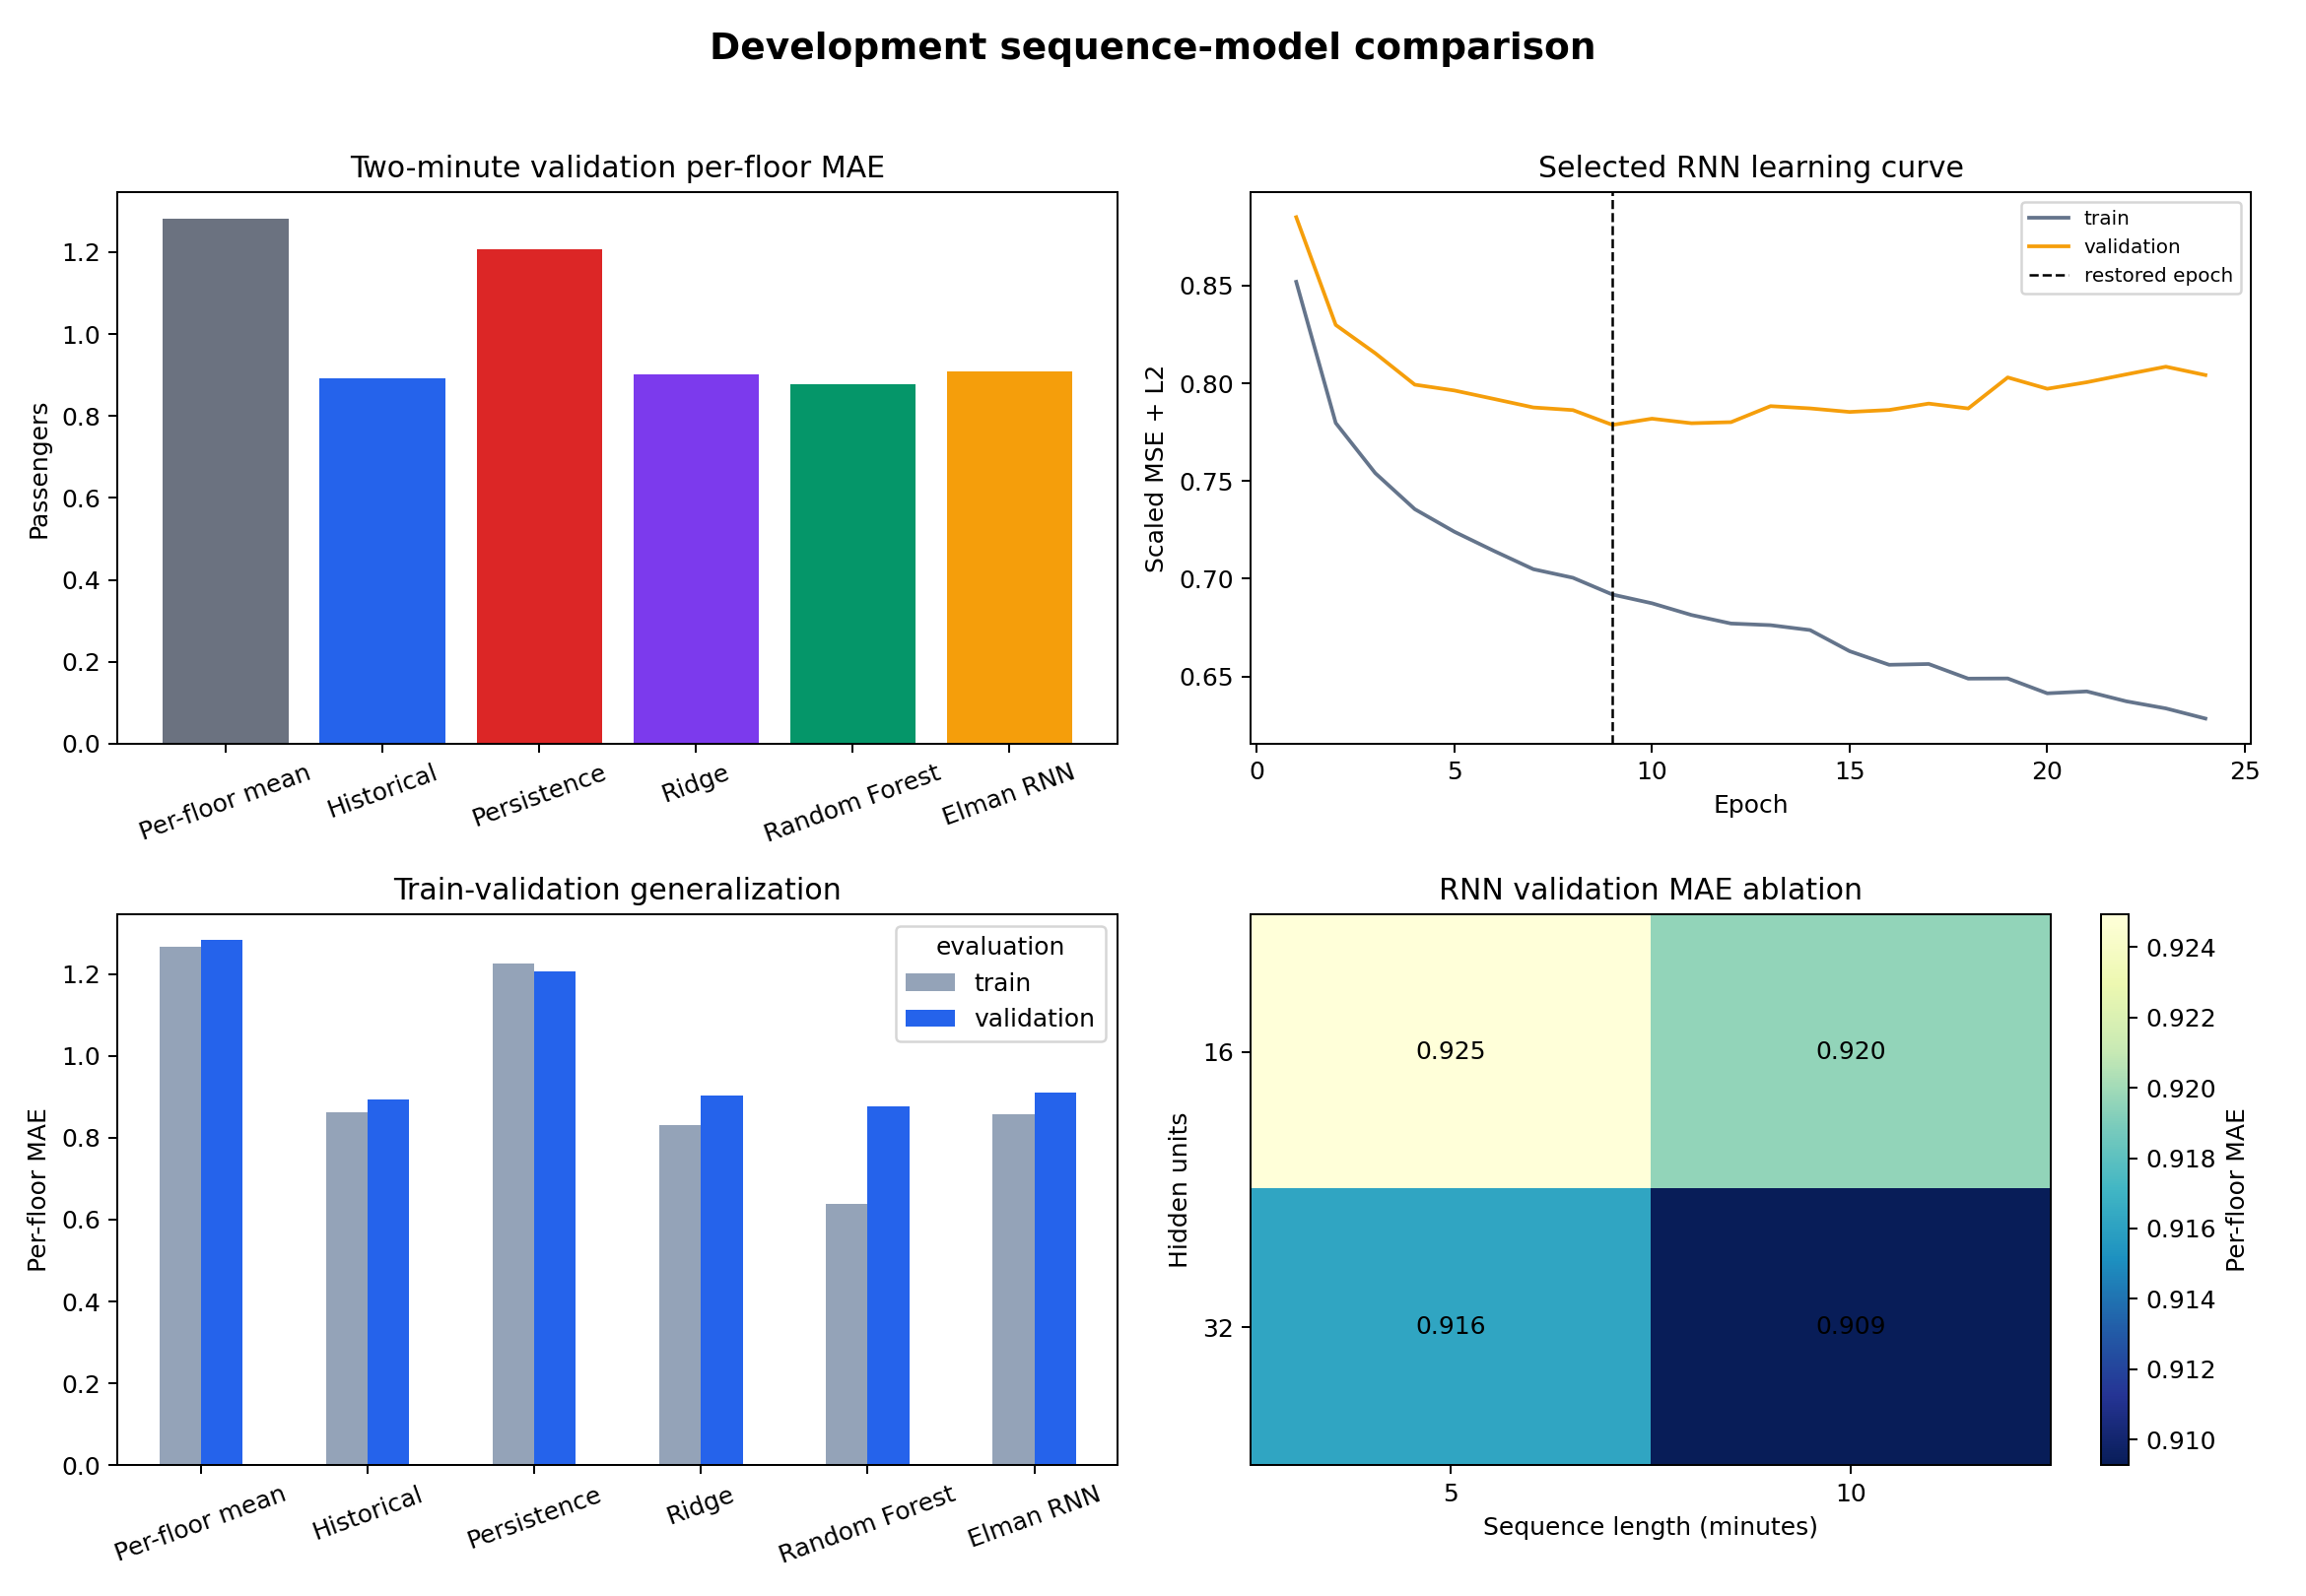
\includegraphics[width=0.96\textwidth]{../results/figures/sequence_model_comparison.png}
  \caption{Development-only model selection diagnostics. Random Forest has the
  lowest validation per-floor MAE, the selected RNN restores epoch 9 as
  validation loss separates from training loss, and the 10-minute, 32-unit RNN
  is the best of the four tested recurrent architectures.}
  \label{fig:development-model-selection}
\end{figure}

Impurity-based interpretation shows that the three- and five-minute lobby
histories have importances 0.304 and 0.255, followed by elapsed-session fraction
at 0.093. This agrees with the lobby-heavy synthetic traffic but also warns
that aggregate accuracy can hide errors on upper floors. The importance is
descriptive, not causal, so floor-level errors and operational simulation
remain necessary. All 12 targeted forecasting, RNN, metric, and protocol tests
passed when this section was prepared.

% Evidence audit: report/evidence/06_controller_methodology.md
\section{Controller Design and Validation-Based Tuning}
\label{sec:controller-methodology}

\subsection{Separating Hall-Call Assignment from Idle-Car Positioning}

Every controller comparison uses the same reactive hall-call assignment rule.
Only the optional positioning policy changes. This separation is necessary:
otherwise a result attributed to forecasting could instead come from a better
assignment heuristic. When a passenger arrives, the nearest-car policy scores
each non-full elevator using the components in
Table~\ref{tab:assignment-score}. The lowest score wins, with elevator ID as a
deterministic tie-breaker.

\begin{table}[H]
  \centering
  \caption{Components of the common hall-call assignment score. All floors,
  stops, and passengers are evaluated from the current simulator state.}
  \label{tab:assignment-score}
  \begin{tabular}{@{}>{\raggedright\arraybackslash}p{0.28\textwidth}
    >{\raggedright\arraybackslash}p{0.62\textwidth}@{}}
    \toprule
    Component & Implemented cost or bonus \\
    \midrule
    Pickup distance & Two seconds per floor between the car and origin. \\
    Existing route & Four seconds for every current service stop. \\
    Assigned queue & 0.75 seconds for every assigned waiting passenger. \\
    Occupancy & 0.5 seconds for every onboard passenger. \\
    Moving away & Twice the time needed to reach the most distant current
      stop, added when the car is travelling away from the new origin. \\
    Existing origin stop & Four-second bonus when the origin is already a
      scheduled stop. \\
    Available at origin & Three-second bonus when a non-moving car is already
      at the origin. \\
    \bottomrule
  \end{tabular}
\end{table}

Assignment immediately cancels the selected car's speculative parking target.
At a pickup, passengers board by arrival time and passenger ID until the
12-person capacity is reached; overflow returns to the global assignment
queue. Consequently, positioning can change where an idle car waits but cannot
override passenger service. This policy is a reproducible benchmark rather
than a claim of commercial optimality: it does not jointly optimize routes,
reserve capacity for assigned passengers, or use destinations before boarding.

\subsection{Positioning Policies and Greedy Decision Rule}

A car is \emph{service-idle} when it has no stops, no assigned waiting
passengers, no onboard passengers, and no active door timer. Static zoning
checks such cars once per minute and sends the four elevators to evenly spaced
floors 0, 5, 9, and 14. The reactive nearest-car baseline supplies no parking
target, so a service-idle car remains where its last trip ended.

Forecast positioning operates at a tunable interval $K$. Let
$\widehat{y}_{t,f}$ be predicted origin demand on floor $f$ during the next two
minutes, let $q_e$ be the current floor of idle elevator $e$, and let $r_f$ be
the number of earlier cars assigned to floor $f$ during the same positioning
update. Candidate floors receive the score

\begin{equation}
  S_{e,f}=\frac{\widehat{y}_{t,f}}{1+r_f}
    -\lambda\lvert f-q_e\rvert,
  \label{eq:positioning-score}
\end{equation}

where $\lambda$ penalizes speculative travel. Cars are processed in elevator-ID
order. A car moves to the first maximum-scoring floor only when that floor
improves on its current-floor score by at least the minimum advantage $\delta$;
otherwise its parking target is cleared. The reservation divisor discourages,
but does not forbid, multiple idle cars from choosing the same floor. No
positioning action is taken when predicted building-wide demand is below 0.5
passengers. The selected settings are $\lambda=0$, $\delta=0.5$, and $K=5$
minutes, so movement is controlled by the five-minute interval and score
threshold rather than an explicit distance term.

The first 10 minutes of each Ridge or Random-Forest schedule use historical
predictions because the learned features do not yet have their maximum required
history. The final protocol retains the policy roles in
Table~\ref{tab:final-controller-policies}. Each forecast-driven row uses the
same score in Equation~\ref{eq:positioning-score} and the same locked settings.

\begin{table}[H]
  \centering
  \caption{Controller policies retained in the sealed final comparison.}
  \label{tab:final-controller-policies}
  \begin{tabular}{@{}>{\raggedright\arraybackslash}p{0.24\textwidth}
    >{\raggedright\arraybackslash}p{0.28\textwidth}
    >{\raggedright\arraybackslash}p{0.38\textwidth}@{}}
    \toprule
    Policy & Positioning input & Scientific role \\
    \midrule
    Nearest car & None & Reactive primary baseline with the common assignment
      rule. \\
    Static zoning & Fixed floors & Non-predictive anticipatory baseline. \\
    Historical positioning & Training schedule means & Tests whether a simple
      demand schedule is enough for control. \\
    Tuned Random Forest & Locked forest predictions & Primary learned
      controller comparison. \\
    Perfect-input greedy & Realized next-two-minute origin counts & Diagnoses
      the shared greedy positioning layer under exact demand input; it is not
      an optimal-control upper bound. \\
    \bottomrule
  \end{tabular}
\end{table}

\subsection{Controller Ablation and Selection Rule}

An exploratory every-minute controller reduced validation mean wait but raised
movement by 7.56\% relative to nearest car. This motivated an explicit
validation-only ablation over

\begin{equation}
  \lambda\in\{0,0.15,0.35,0.60\},\quad
  \delta\in\{0,0.5,1.0\},\quad
  K\in\{1,2,5\}\ \text{minutes},
  \label{eq:controller-grid}
\end{equation}

for 36 configurations. Each configuration was simulated on the same 12
validation days and paired against nearest car. The predeclared movement budget
allowed at most 5\% additional floors travelled. Within that budget, the strict
rule required lower mean wait and no increase in day-averaged P95 wait, then
maximized mean-wait savings. If no candidate met all constraints, the relaxed
rule minimized P95 change within budget, using mean-wait savings and movement
as tie-breakers.

No grid candidate passed every strict service constraint. Twenty-eight were
within the movement budget, and the relaxed rule selected
$(\lambda,\delta,K)=(0,0.5,5)$. Its validation diagnostics are shown in
Table~\ref{tab:controller-selection}. Because these 12 days selected both the
forecast model and the controller, the values are development evidence rather
than unbiased performance estimates.

\begin{table}[H]
  \centering
  \caption{Validation diagnostics for the locked controller. Positive
  mean-wait savings favor the candidate; positive P95 or movement changes
  indicate a cost relative to nearest car.}
  \label{tab:controller-selection}
  \begin{tabular}{@{}lr@{}}
    \toprule
    Quantity & Validation value \\
    \midrule
    Mean wait & 15.245 s \\
    Mean-wait savings & 0.382 s \\
    P95 wait & 49.471 s \\
    P95 change & $+0.008$ s \\
    Mean floors travelled per day & 3725.5 \\
    Paired movement change & $+1.35\%$ \\
    Days with lower mean wait & 7 of 12 \\
    \bottomrule
  \end{tabular}
\end{table}

The selected controller was then challenged on development-only unseen-surge
and 1.5-times-demand days without further parameter tuning. Figure
\ref{fig:controller-ablation} records both the selection landscape and those
stress diagnostics. The surge result is intentionally unfavorable: it reveals
that a controller can obey its movement budget on normal validation traffic
yet fail under a changed arrival pattern.

\begin{figure}[H]
  \centering
  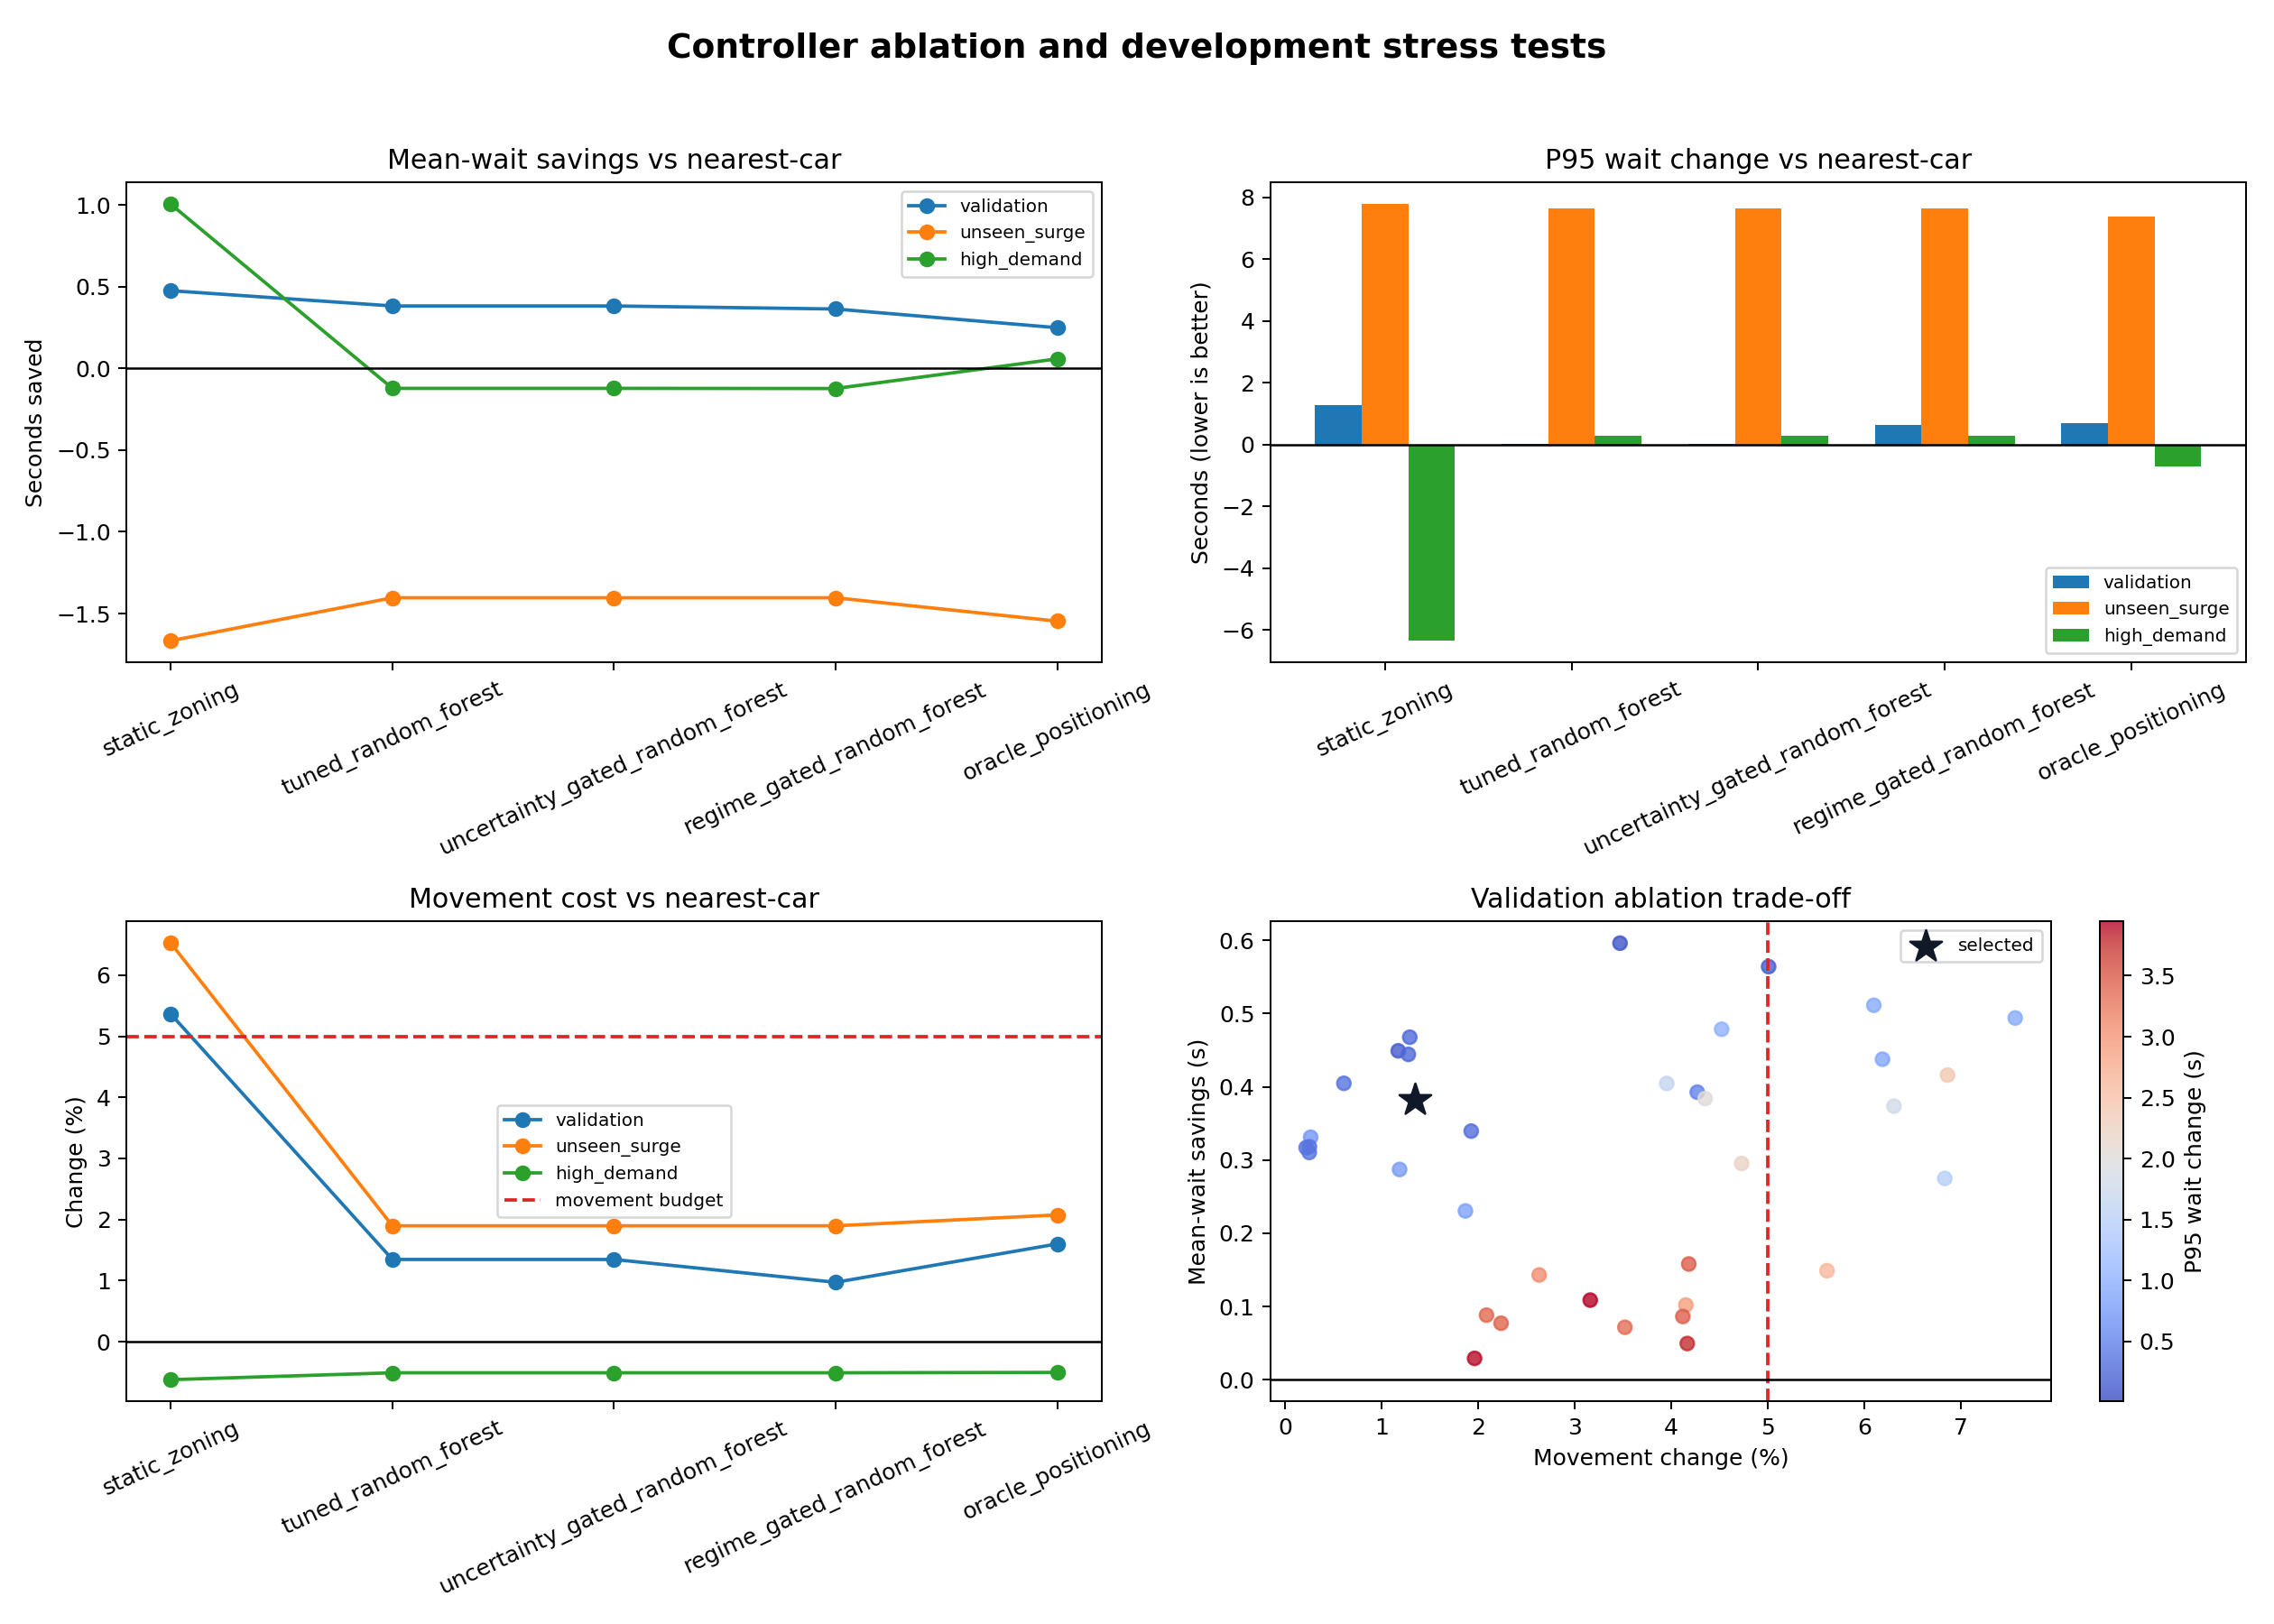
\includegraphics[width=0.96\textwidth]{../results/figures/robustness_comparison.png}
  \caption{Development-only controller ablation and stress diagnostics. The
  star identifies the locked configuration and the dashed line is the 5\%
  movement budget. The legacy plot label ``oracle positioning'' denotes the
  perfect-input greedy diagnostic, not an optimal controller. None of these
  stress days belongs to the final holdout.}
  \label{fig:controller-ablation}
\end{figure}

\subsection{Service Metrics, Pairing, and Diagnostic Gates}

Passenger wait is boarding time minus arrival time; ride time is drop-off minus
boarding; and journey time is drop-off minus arrival. The primary controller
metric is day-level mean passenger wait. Secondary service diagnostics are P95
wait, the fraction waiting more than 60 seconds, mean journey time, and the
gap between the largest and smallest observed origin-floor mean waits. Floors
travelled is the primary movement-cost proxy; stops, reversals, peak load,
unserved passengers, and post-generation drain time are retained as operational
checks. Metrics are emitted only after every generated passenger is served.

Comparisons are paired by building day, so each candidate receives exactly the
same passenger stream as its baseline. For lower-is-better metrics, reported
savings are baseline minus candidate. The 95\% percentile intervals resample
these paired day differences 2,000 times with fixed seeds. This preserves the
building day, rather than a correlated passenger or minute, as the independent
unit. The 5\% movement budget is a development selection constraint and a proxy
for operating cost; it is not a direct energy measurement or safety guarantee.

Two additional development gates were investigated but excluded from the final
policy list. An uncertainty gate disabled positioning above the validation
90th percentile of mean Random-Forest tree disagreement. At the selected
five-minute decision times it made the same decisions as the always-on forest,
so it provided no distinct final comparison and should not be interpreted as
calibrated uncertainty. A regime gate disabled positioning for the synthetic
mixed-traffic label, but that exact generator label would not be available in a
real building and was therefore not treated as deployable.

Finally, perfect-input greedy positioning receives the realized future origin
counts but retains the same sequential heuristic. If it improves service while
the learned controller does not, forecast error is a plausible bottleneck; if
even perfect input fails, the evidence instead points toward the positioning
logic or its objective. This classification is diagnostic, not causal, because
the perfect-input controller is destination-unaware and does not optimize a
joint route, capacity, fairness, or tail-wait objective.

All 20 targeted controller, metric, selection, and diagnostic tests passed.
The complete 74-test regression suite also passed after the section was
prepared.

% Evidence audit: report/evidence/07_final_results.md
\section{Untouched Final-Holdout Results}
\label{sec:final-results}

\subsection{Chain of Custody and Evaluation Sample}

The final protocol was locked on August 10, 2026 at 17:37:49 UTC. Seed offset
16,575,894 was revealed the next day at 23:21:44 UTC, after which the guarded
runner executed once and completed at 23:22:16 UTC. It generated 20
in-distribution days, eight unseen-surge days, and eight 1.5-times-demand days.
These 36 independent days contain 31,820 passengers and produce 216 model-day
rows and 180 policy-day rows. Passenger streams are identical across policies
within a day, every passenger is served, and peak car load never exceeds
capacity.

The saved configuration, protocol, and seed snapshots are semantically equal
to their active JSON files, and every entry in the immutable final-artifact
manifest verifies. A post-run type-only import-order correction changed the
active hash of \texttt{policies.py}; it changes annotation imports but no score,
decision, model, or metric logic. The holdout was not rerun. Therefore the
pre-run source manifest now has one explicitly documented mismatch, while all
seeds, fitted models, result tables, snapshots, completion metadata, and the
final figure retain their original verified hashes.

\subsection{Forecasting Performance}

Table~\ref{tab:final-forecast-all} compares all six locked forecasters. Random
Forest has the lowest in-distribution MAE at 0.868, but the best model changes
under distribution shift: persistence is best on the unseen surge and Ridge is
best under 1.5-times demand. Thus no single architecture dominates every
traffic condition.

\begin{table}[H]
  \centering
  \caption{Final two-minute per-floor MAE. Lower is better; bold values are the
  best within each independently generated evaluation.}
  \label{tab:final-forecast-all}
  \begin{tabular}{@{}lrrr@{}}
    \toprule
    Model & In distribution & Unseen surge & 1.5x demand \\
    \midrule
    Per-floor mean & 1.279 & 1.706 & 1.623 \\
    Historical mean & 0.897 & 1.657 & 1.240 \\
    Persistence & 1.224 & \textbf{1.476} & 1.539 \\
    Ridge & 0.881 & 2.365 & \textbf{1.094} \\
    Random Forest & \textbf{0.868} & 1.642 & 1.162 \\
    Elman RNN & 0.905 & 1.630 & 1.221 \\
    \bottomrule
  \end{tabular}
\end{table}

The locked primary comparison is Random Forest against historical mean. Its
day-paired effects in Table~\ref{tab:final-forecast-effects} define positive
values as an MAE reduction. In distribution, the reduction is 0.028 passengers
with a 95\% interval of [0.011, 0.046], and the forest wins 14 of 20 days. This
supports the primary forecasting hypothesis, although the magnitude is small.
The Elman RNN does not beat historical mean: its MAE is 0.905 versus 0.897, and
its paired reduction is $-0.008$ with interval [$-0.025$, 0.009].

\begin{table}[H]
  \centering
  \caption{Paired Random-Forest MAE reduction relative to historical mean.
  Intervals resample independent building days 2,000 times.}
  \label{tab:final-forecast-effects}
  \begin{tabular}{@{}lrrrrr@{}}
    \toprule
    Evaluation & Hist. & Forest & Reduction & 95\% interval & Wins \\
    \midrule
    In distribution & 0.897 & 0.868 & 0.028 & [0.011, 0.046] & 14/20 \\
    Unseen surge & 1.657 & 1.642 & 0.015 & [$-0.009$, 0.041] & 4/8 \\
    1.5x demand & 1.240 & 1.162 & 0.078 & [0.037, 0.126] & 7/8 \\
    \bottomrule
  \end{tabular}
\end{table}

The surge interval includes zero, so the forest's 0.015 advantage is
inconclusive; persistence instead improves on historical mean by 0.181 with an
interval of [0.144, 0.218]. Ridge degrades to 2.365 MAE and has positive bias
0.819, showing a severe extrapolation failure. Under higher demand, Random
Forest retains a stable advantage over historical mean, but Ridge is best
overall at 1.094 MAE. These shifts justify reporting the complete comparison
rather than declaring Random Forest universally robust.

\subsection{In-Distribution Controller Performance}

The operational conclusion differs from the forecast conclusion. As shown in
Table~\ref{tab:final-controller-all}, Random-Forest positioning changes mean
wait from 16.023 to 16.038 seconds, P95 wait from 52.413 to 53.580 seconds, and
movement from 3,720 to 3,780 floors per day. Its paired mean-wait savings are
$-0.015$ seconds with interval [$-0.485$, 0.394], and it wins exactly 10 of 20
days. The primary controller hypothesis is therefore not supported.

\begin{table}[H]
  \centering
  \caption{In-distribution controller results averaged over 20 independent
  days. Long wait is the percentage above 60 seconds.}
  \label{tab:final-controller-all}
  \begin{tabular}{@{}lrrrrr@{}}
    \toprule
    Policy & Mean wait & P95 & Long wait & Fairness gap & Movement \\
    \midrule
    Nearest car & 16.023 & 52.413 & 4.05\% & 19.203 & \textbf{3,720} \\
    Static zoning & \textbf{15.510} & \textbf{51.635} & \textbf{3.77\%} &
      \textbf{17.139} & 3,928 \\
    Historical positioning & 16.086 & 53.650 & 4.09\% & 20.024 & 3,779 \\
    Random-Forest positioning & 16.038 & 53.580 & 4.03\% & 20.006 & 3,780 \\
    Perfect-input greedy & 15.651 & 52.558 & 3.82\% & 19.065 & 3,789 \\
    \bottomrule
  \end{tabular}
\end{table}

Static zoning has the best average service metrics and saves 0.513 seconds of
mean wait, but its interval [$-0.148$, 1.242] includes zero and its 5.73\%
movement increase exceeds the locked 5\% development budget. Perfect-input
greedy saves 0.372 seconds with interval [$-0.186$, 0.933], but worsens P95 by
0.145 seconds. Exact future origin counts are therefore insufficient to make
the shared greedy positioner reliably beneficial.

\subsection{Distribution-Shift Controller Results}

Table~\ref{tab:final-controller-effects} extends the primary Random-Forest
comparison to both stress conditions. Neither establishes a robust mean-wait
improvement. The surge estimate is positive but highly uncertain. The
high-demand interval misses excluding zero by 0.0005 seconds, and only three of
eight days have lower mean wait despite favorable mean and P95 estimates.

\begin{table}[H]
  \centering
  \caption{Paired Random-Forest controller effects versus nearest car. Positive
  wait savings favor positioning; positive movement is additional travel.}
  \label{tab:final-controller-effects}
  \begin{tabular}{@{}lrrrrr@{}}
    \toprule
    Evaluation & Mean saved & 95\% interval & P95 saved & Movement & Wins \\
    \midrule
    In distribution & $-0.015$ & [$-0.485$, 0.394] & $-1.168$ & +1.75\% & 10/20 \\
    Unseen surge & 0.147 & [$-1.218$, 1.726] & 1.131 & +0.37\% & 4/8 \\
    1.5x demand & 0.369 & [$-0.001$, 0.934] & 2.650 & +0.11\% & 3/8 \\
    \bottomrule
  \end{tabular}
\end{table}

Historical and Random-Forest positioning produce exactly identical complete
metric rows on every final surge and high-demand day. Different prediction
errors can therefore collapse to the same actions after the five-minute
schedule, reservation rule, and 0.5 score threshold. Figure
\ref{fig:final-comparison} visualizes the resulting disconnect: forecast gains
and controller gains are different quantities and can move in opposite
directions.

\begin{figure}[H]
  \centering
  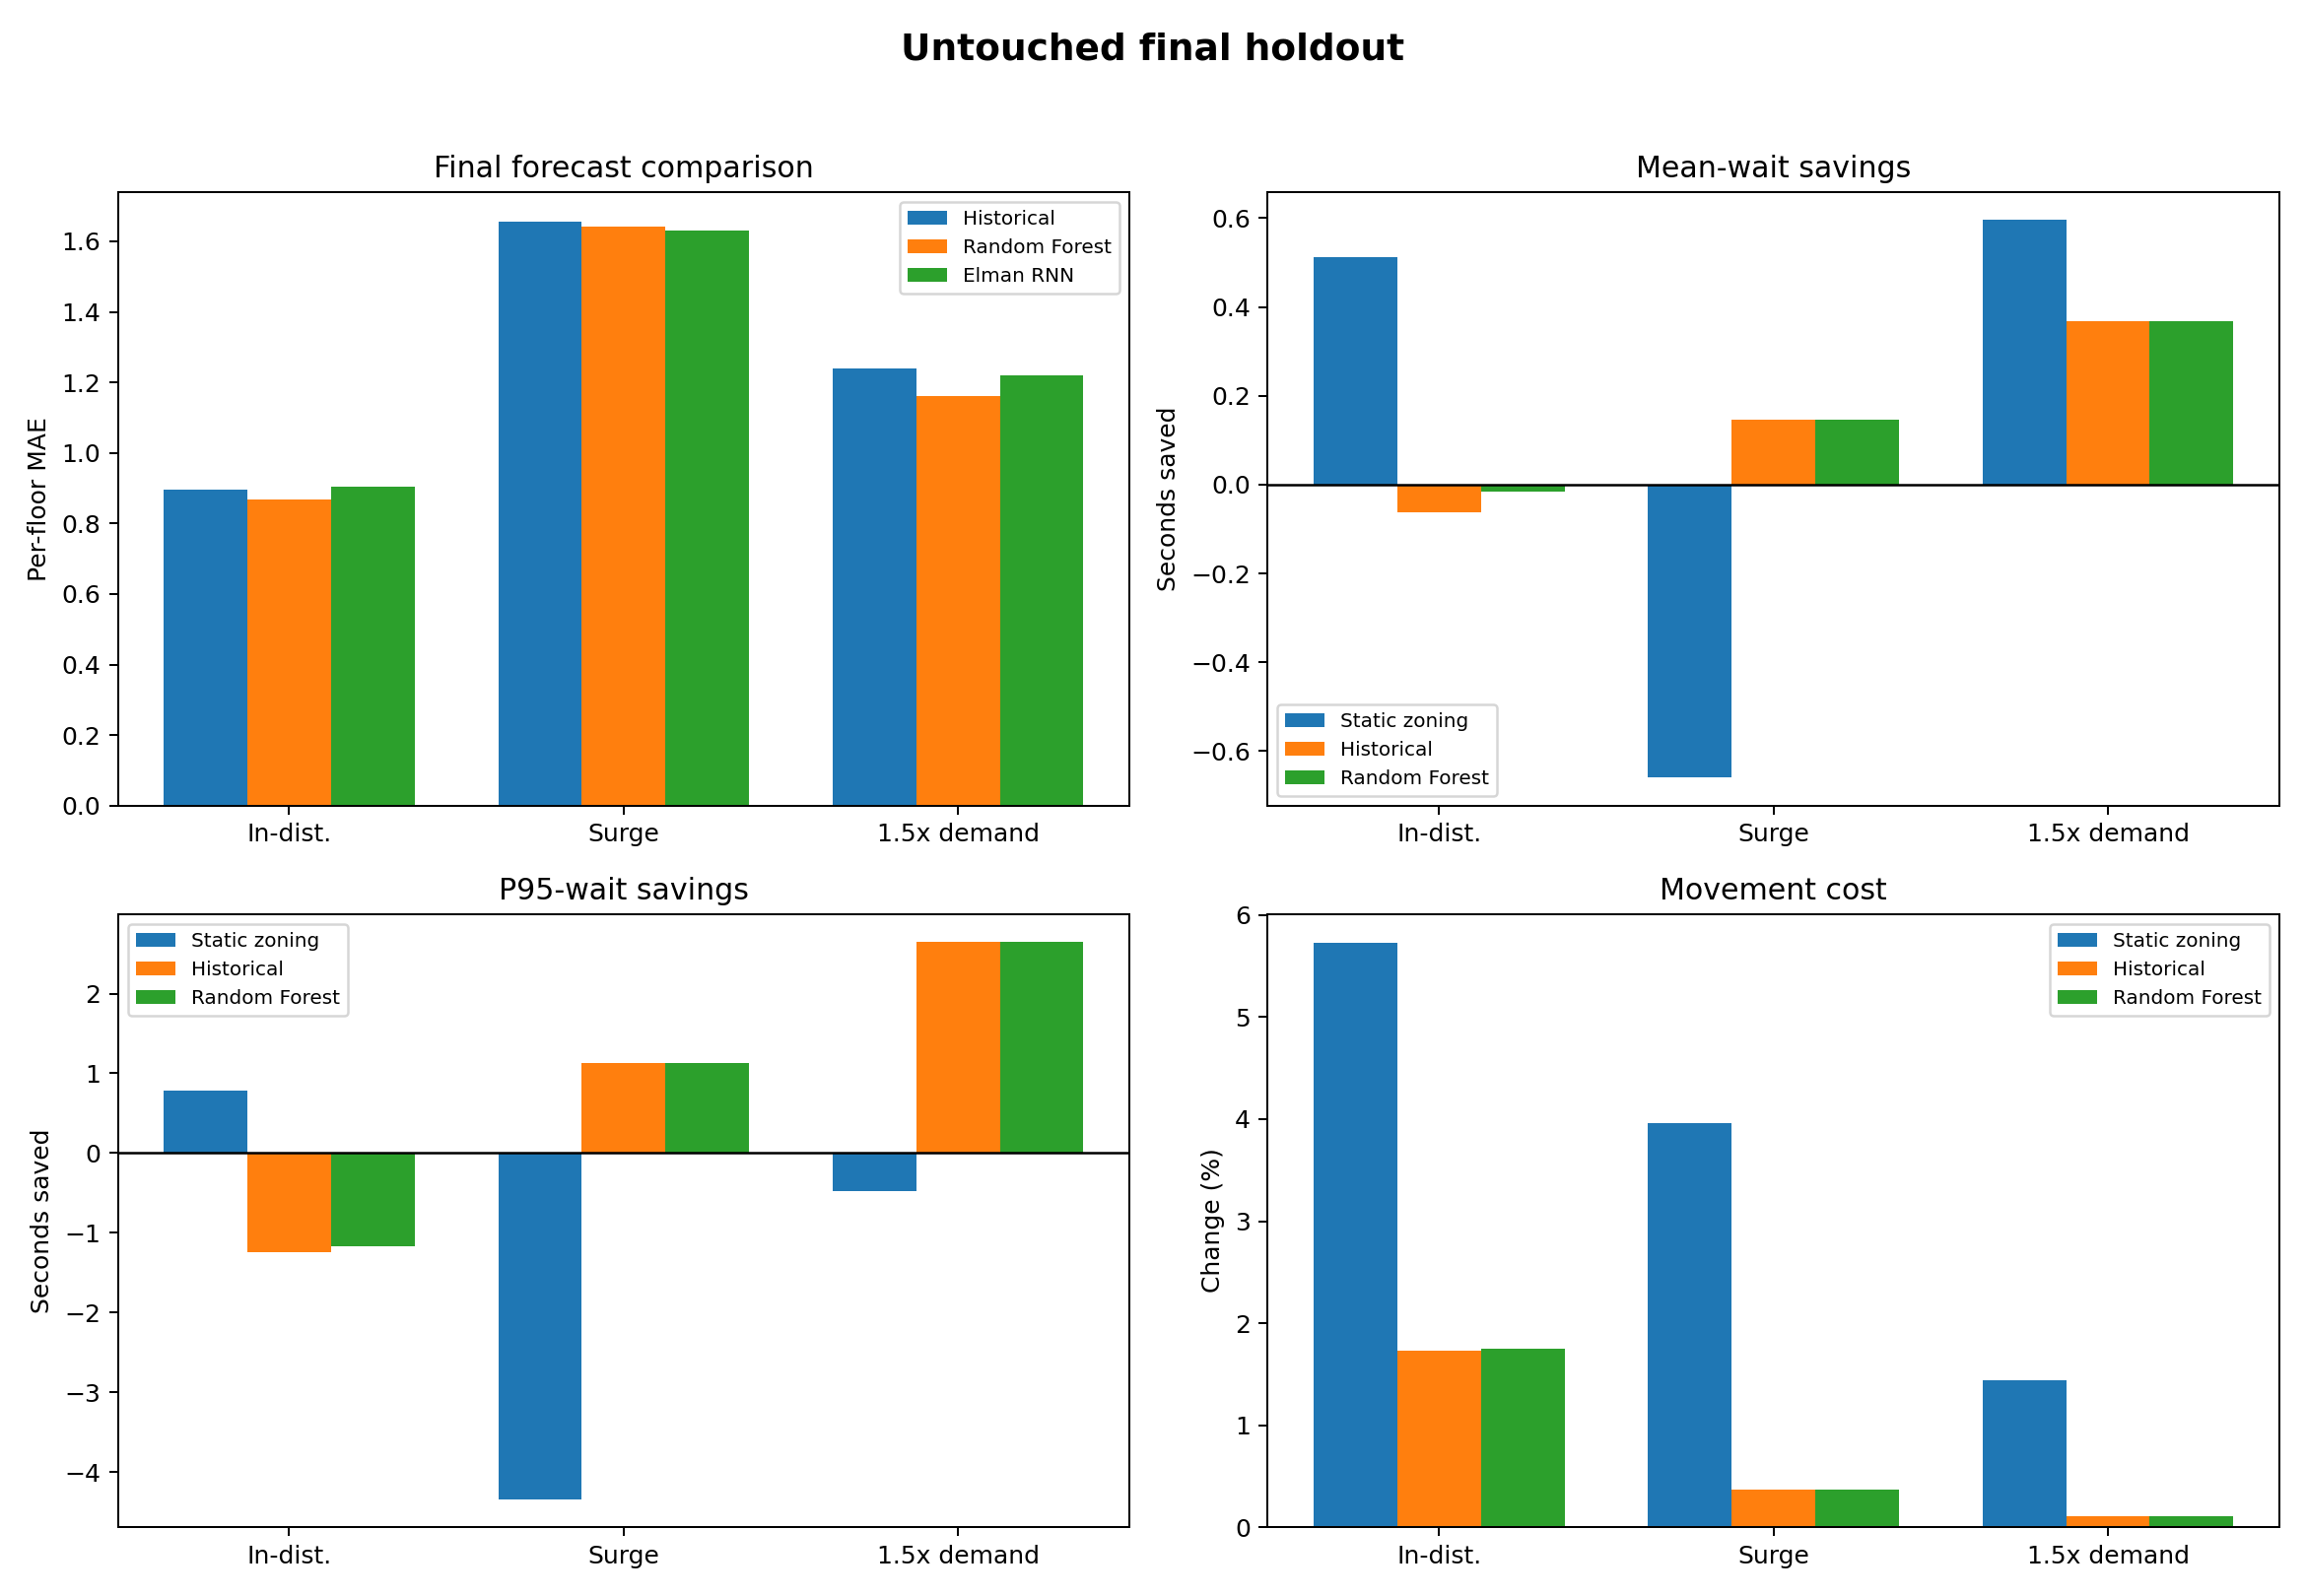
\includegraphics[width=0.96\textwidth]{../results/figures/final_comparison.png}
  \caption{Forecast and controller results on the untouched final holdout.
  Forecast MAE is lower-is-better; controller panels show savings relative to
  nearest car and paired movement change. Random Forest improves prediction
  without delivering a reliable in-distribution operational advantage.}
  \label{fig:final-comparison}
\end{figure}

\subsection{Scenario and Floor Diagnostics}

The in-distribution scenario slice in Table~\ref{tab:final-scenario-slice} is
descriptive and was not used for further tuning. Lunch supplies the forest's
largest forecast gain and five wins in five days, yet mean wait worsens by
0.111 seconds. Morning P95 worsens by 5.50 seconds while movement rises 4.31\%.
Evening is the only scenario with positive average mean-wait savings, despite
almost no forecast-MAE advantage.

\begin{table}[H]
  \centering
  \caption{Exploratory Random-Forest effects by in-distribution traffic
  scenario. Positive savings favor Random Forest; movement is additional.}
  \label{tab:final-scenario-slice}
  \begin{tabular}{@{}lrrrr@{}}
    \toprule
    Scenario & Forecast MAE saved & Mean wait saved & P95 saved & Movement \\
    \midrule
    Morning & 0.018 & $-0.089$ & $-5.500$ & +4.31\% \\
    Lunch & 0.089 & $-0.111$ & $-0.270$ & +2.19\% \\
    Evening & 0.005 & 0.194 & 0.280 & +0.13\% \\
    Mixed & 0.001 & $-0.054$ & 0.820 & +0.37\% \\
    \bottomrule
  \end{tabular}
\end{table}

The floor slice reveals that the forecast gain is spatially concentrated. The
lobby alone reduces MAE by 0.388; because the overall metric equally averages
15 floors, this contributes approximately 91\% of the net 0.028 reduction.
Forest MAE instead worsens by 0.022 on floor 5 and 0.018 on floor 13.
Passenger-weighted controller results are also heterogeneous: the largest wait
savings occur on floors 3 and 10 (0.884 and 0.627 seconds), while floors 1 and
14 lose 0.643 and 0.480 seconds. These post-hoc extremes have no
multiplicity-adjusted inference and should be read as failure-analysis clues,
not new hypotheses.

Overall, the primary forecasting hypothesis is supported, while the primary
controller hypothesis is not. The secondary tail, fairness, and movement
evidence also prevents describing the learned positioner as an operational
improvement. Stress and slice results reinforce the need to evaluate the
forecast-to-action mapping rather than infer system value from offline MAE.

% Evidence audit: report/evidence/08_discussion_limitations.md
\section{Discussion, Limitations, and Future Work}
\label{sec:discussion}

\subsection{Interpretation of the Main Finding}

The forecasting and controller hypotheses measure different pipeline stages.
Random Forest reduces in-distribution per-floor MAE by 0.028 passengers, but a
prediction changes service only when a car is idle, a five-minute update occurs,
and the best-floor advantage reaches 0.5. Improvements that do not cross these
boundaries produce no action, while a small error that does can trigger a
harmful move. Offline MAE can compare predictors but cannot select a controller
without operational evaluation.

The gain is also concentrated: the lobby contributes about 91\% of the net MAE
reduction, while floor wait effects have both signs and the mean fairness gap
worsens by 0.803 seconds. The Elman RNN's 0.905 MAE does not beat the 0.897
historical baseline, so its tested complexity is not justified here. Conversely,
static zoning achieves the lowest average wait without learning, although its
interval includes zero and movement exceeds budget. These results show why
strong heuristics and spatial service diagnostics must accompany model metrics.

\subsection{Failure-Mode Analysis}

Four observations localize the failure. First, lobby-dominated MAE is poorly
aligned with upper-floor coverage. Second, five-minute sampling and the score
threshold compress different forecasts into identical actions: historical and
forest controllers match on all 16 final stress days. Third, perfect-input
greedy remains inconclusive and slightly worsens P95, exposing the shared
origin-only, destination-unaware objective. Fourth, static zoning's lower mean
wait costs 5.73\% extra movement, so service and operating cost cannot be
optimized independently.

A descriptive perfect-input classification gives 10 benefit-realized, three
forecast-limited, and seven controller-limited in-distribution days. Five of
eight surge and four of eight high-demand days are controller-limited. These
labels are not causal, but they show that replacing the forecaster alone is
insufficient. The uncertainty gate also does not repair the system: uncalibrated
tree disagreement rarely peaks at decision times, so gated and ungated
controllers take identical development actions.

\subsection{Limitations and Threats to Validity}

The paired seeded design isolates policy differences inside the digital twin,
but it cannot establish real-building effectiveness. Table
\ref{tab:validity-threats} summarizes the claim boundaries.

\begin{table}[H]
  \centering
  \caption{Principal limitations and consequences for interpretation.}
  \label{tab:validity-threats}
  \begin{tabular}{@{}>{\raggedright\arraybackslash}p{0.20\textwidth}
    >{\raggedright\arraybackslash}p{0.70\textwidth}@{}}
    \toprule
    Threat & Boundary and consequence \\
    \midrule
    External validity & Synthetic traffic, one 15-floor/four-car building, and
      fixed regimes require calibration before transfer to a real building. \\
    Simulator fidelity & Constant kinematics and instantaneous boarding omit
      obstruction, abandonment, failures, priority, freight, accessibility,
      and emergency modes; seconds are comparative, not certified predictions. \\
    Controller scope & Origin-only greedy parking lacks joint route, destination,
      capacity, and tail-service optimization; this is not complete group control. \\
    Construct validity & Floors travelled is not calibrated energy, and the
      max-min floor-wait gap is location-based service disparity, not
      demographic fairness. \\
    Statistical validity & Only 20 primary and eight days per stress set are
      available; stress intervals are wide and post-hoc slices have no
      multiplicity-adjusted inference. \\
    Drift and sensing & Two synthetic shifts omit missing, delayed, or noisy
      counts, while tree disagreement is uncalibrated. \\
    Reproducibility & Final artifacts remain immutable, but exact source lineage
      includes the disclosed post-run type-only hash change. \\
    \bottomrule
  \end{tabular}
\end{table}

No identity or demographic attributes are generated. This reduces privacy
exposure but prevents protected-group fairness or accessibility claims. Real
deployment requires data minimization, retention and access controls, and
metrics defined with affected users. Likewise, the confidence intervals cover
sampled-day variation conditional on fixed simulator assumptions; they do not
include uncertainty in human behavior, building geometry, timing, or the
controller objective.

\subsection{Prioritized Future Work}

Future work should improve the weakest layer before enlarging the predictor:

\begin{enumerate}[leftmargin=0.34in,itemsep=0.20em,topsep=0.20em]
  \item \textbf{Calibrate with real data.} Fit anonymous aggregate arrival, OD,
    door, and travel distributions from multiple buildings, reserving later
    periods or buildings as holdouts. Baseline service should match measured
    ranges before policy claims.
  \item \textbf{Redesign control.} Add destination-aware route insertion,
    capacity planning, and a receding-horizon objective for mean wait, P95,
    fairness, and movement. The gate is whether perfect-input control improves
    both mean and P95 within budget.
  \item \textbf{Align prediction with decisions.} Predict OD flows or demand
    quantiles, optimize an action-level loss, and calibrate uncertainty at
    actual decision times with zoning as an abstention policy.
  \item \textbf{Broaden robustness.} Vary floors, cars, capacity, kinematics,
    and horizon; inject sensor delay and missingness; add calibrated energy and
    shadow-mode monitoring. Benefits must persist without capacity, tail-wait,
    or energy regressions.
\end{enumerate}

Priority 2 is the immediate research gate: if redesigned control cannot turn
perfect demand into reliable value, additional forecasting complexity is
unlikely to help.

% Evidence audit: report/evidence/09_conclusion_contributions.md
\section{Conclusion}
\label{sec:conclusion}

This project asked whether leakage-safe short-horizon demand forecasting can
improve multi-elevator service under normal traffic and distribution shift. It
answered that question through a complete applied-ML workflow: a validated
digital twin, independent building-day splits, six forecasting models, five
controller policies, a from-scratch RNN, validation-only model and controller
selection, ablations, paired uncertainty intervals, stress tests, floor-level
diagnostics, and a sealed run-once final holdout.

The four locked research questions have direct answers. \textbf{RQ1: yes.}
Random Forest reduces in-distribution per-floor MAE from 0.897 to 0.868; the
paired reduction is 0.028 with 95\% interval [0.011, 0.046]. \textbf{RQ2: no.}
Its controller changes mean wait from 16.023 to 16.038 seconds, giving
$-0.015$ seconds saved with interval [$-0.485$, 0.394]. \textbf{RQ3: no safe
operational benefit is established.} P95 wait worsens by 1.168 seconds,
fairness gap rises by 0.803 seconds, and movement rises by 1.75\% in
distribution. Static zoning has the best average service but exceeds the
movement budget, while perfect-input greedy remains inconclusive. \textbf{RQ4:
the conclusion is shift-dependent but not reversed.} Persistence is the best
surge forecaster and Ridge is best at 1.5-times demand; Random-Forest
positioning establishes no robust mean-wait improvement in either stress set.

The main engineering lesson is that better prediction is not equivalent to
better control. Forecasts matter only through the actions, constraints, and
objective of the downstream decision layer. In this system, thresholded
five-minute decisions, origin-only information, and greedy positioning discard
or misuse part of the predictive gain. The negative controller result is
therefore substantive: it identifies where the next engineering effort should
go and prevents an offline accuracy improvement from being overstated as a
deployable service improvement.

\section{Team Contributions}

Hannah Abedin and Erfan Razmand developed the project with shared ownership
across problem formulation, system design, implementation review, leakage
validation, experimentation, interpretation, writing, reproducibility, and
presentation. The authors jointly stand behind the implementation, analysis,
and reported conclusions; no subsystem or result is assigned as the exclusive
work of either author.

\section{Acknowledgements and Tool Use}

EECS 3404 lecture materials provided instructional context
\cite{eecs3404materials2026}. The code uses NumPy, pandas, scikit-learn, joblib,
and Matplotlib
\cite{harris2020numpy,mckinney2010pandas,pedregosa2011scikit,hunter2007matplotlib}.
OpenAI Codex assisted with scaffolding, code/prose drafts, checks, and evidence
organization. Both authors reviewed the work and retain responsibility. No
external inference API or pretrained model generated the predictions or results.

\clearpage
\bibliographystyle{plain}
\bibliography{references}

\end{document}
